
\documentclass[a4paper,12pt,parskip,bibtotoc,liststotoc]{article}
    %Festlegung der Dokumentenklasse, zahlreiche Vereinbarungen über Layout, Gliederungsstrukturen,
    %bsp. article -> section, subsection..., book -> chapter, section...
    %parskip = Abstand zwischen Absätzen, Veränderung durch \setlength

\usepackage[ngerman]{babel}     %Neue deutsche Rechtschreibung, Umlaute können geschrieben werden
\usepackage[utf8]{inputenc}     %direkte Angabe von Umlauten
\usepackage[T1]{fontenc}        %Silbentrennung bei Sonderzeichen
\usepackage{setspace}           %für Zeilenabstand
\usepackage[notindex,nottoc]{tocbibind}   %Inhaltsverzeichnisse erstellen


\usepackage{mathptmx,charter,courier} % Für schöne Schriften
\usepackage[scaled]{helvet}     		%Serifenlose Schrift wird in Helvetica geschrieben
\usepackage{calligra}    				%Calligra Schriftart
\usepackage{eufrak}      				%mathematische Symbole


%zusätzliche benötigte Pakete
\usepackage{graphicx}           %Graphik
\usepackage{amsmath}    		%Mathematik
\usepackage{natbib}             %Zitate
\usepackage{marvosym}           %enthält Symbole wie das Eurozeichen
\usepackage{eurosym}

%\setcounter{secnumdepth}{3}
%\setcounter{tocdepth}{3}



\usepackage{mdwlist}   			%Verringerung Abstand zwischen items -> \begin{itemize*} \end{itemize*}
\usepackage[labelsep=space,justification=centering]{caption} % Abbilungd-/Tabellen Über-/Unterschriften

%\usepackage{hyperref}  		%erlaubt Links innerhalb des pdf-Dokuments zu erzeugen

\setlength{\parindent}{0pt}     %Verhinderung des horizontalen Einrückens zu Beginn eines Absatzes

%Seitenlayout
\topmargin -0.9cm       %Vertikaler Abstand der Kopfzeile von der Bezugslinie
\textheight 25cm        %Abstand der Grundlinie der Kopfzeile zum Haupttext
\textwidth 16.5cm       %Breite des Haupttexts
\footskip 1cm           %Abstand der Grundlinien der letzten Textzeile und der Fußzeile
\voffset -0.5cm         %Vertikale Bezugspunktposition
\hoffset -1.2cm         %Horizontale Bezugspunktposition

\onehalfspacing         %anderthalbzeiliger Abstand

\newcommand{\url}{\;}   %URL im Literaturverzeichnis

%eigene Befehlsdefinitionen
\newcommand{\be}{\begin{equation}}     %Mathematische Umgebung
\newcommand{\ee}{\end{equation}}
\newcommand{\bea}{\begin{eqnarray}}
\newcommand{\eea}{\end{eqnarray}}
\newcommand{\bean}{\begin{eqnarray*}}  %ohne Nummerierung
\newcommand{\eean}{\end{eqnarray*}}    %ohne Nummerierung

%%%%%%%%% ACHTUNG, HIER NEU HINZUGEFÜGTE PACKAGES%%%%%%%%%%%%%%%%%%%%%%%%%%%%
%

\usepackage{titlesec} %weitere subsubsubsection

\usepackage{natbib}
\let\bibhang\relax
\let\citename\relax
\let\bibfont\relax
\let\Citeauthor\relax
\expandafter\let\csname ver@natbib.sty\endcsname\relax
\usepackage[backend = bibtex, style = authoryear, doi = false, date = long, isbn = false]{biblatex}

\addbibresource{Literatur2.bib}



\usepackage{listings}

\setcounter{secnumdepth}{4}

\titleformat{\paragraph}
{\normalfont\normalsize\bfseries}{\theparagraph}{1em}{}
\titlespacing*{\paragraph}
{0pt}{3.25ex plus 1ex minus .2ex}{1.5ex plus .2ex}

%
%%%%%%%%%%%%%%%%%%%%%%%%%%%%%%%%%%%%%%%%%%%%%%%%%%%%%%
\begin{document}

\pagenumbering{roman}  %römische Seitennummerierung
%%%%%%%%%%%%%%%%%%%%%%%%%%%%%%%%%%%%%%%%%%%%%%%%%%%%%%
%
%    Titelseite
%
%%%%%%%%%%%%%%%%%%%%%%%%%%%%%%%%%%%%%%%%%%%%%%%%%%%%%%
\thispagestyle{empty}  %keine Seitenzahl auf Titelseite
Leibniz Universität Hannover\\
Wirtschaftswissenschaftliche Fakultät\\
Institut für Produktionswirtschaft\\
Prof.\ Dr.\ Stefan Helber

\vspace{5cm}

\begin{center}
Hausarbeit \\
im Rahmen des Seminars zur Produktionswirtschaft im WS 2016/17 \\
(Veranstaltungs-Nr. 171137)

\vspace{2.5cm}

Thema Nr. ..\\[1mm]    %hier Themennummer eintragen
{\Large Titel }
\end{center}

\vspace{7.5cm}

Vorname Name \\
Straße Hausnummer \\
PLZ Ort \\
Matr.-Nr. 1234567 \\[3mm]
Abgabedatum:


\newpage

%Inhaltsverzeichnis erstellen
\tableofcontents

\newpage  %neue Seite

%Abbildungsverzeichnis erstellen
\listoffigures

%Tabellenverzeichnis erstellen
\listoftables

%Abkürzungsverzeichnis
\section*{Abkürzungsverzeichnis}
\addcontentsline{toc}{section}{Abkürzungsverzeichnis}
\begin{table}[h!]
    \vspace*{-3mm}
    \hspace*{2mm}
  \renewcommand{\arraystretch}{1,5}
    \begin{tabular}{ll}  %hier die Spaltenausrichtung und Anzahl eintragen
FLP & Facility Location Problem\\

VRP &  Vehicle Routing Problem\\

LRP & Location Routing Problem\\

CVRP & Capacitated Vehicle Routing Problem\\

ELRP & Electric Location Routing Problem\\

TSP & Traveling Salesman Problem\\

VRP-TW & Vehicle Routing Problem with Time Windows\\

ELRP-TW & Electric Location Routing Problem with TIme Windows\\

MDVRP & Multi-Depot Vehicle Routing Problem\\

MTVRP & Multi Trip Vehicle Routing Problem \\

ICT-Systems & Information and Communications Technology\\

ca. & circa\\

sog. & sogenannte \\

bzw. & beziehungsweise \\

i.H.v. & in Höhe von\\

bzgl. & bezüglich\\

z.B & zum Beispiel\\

bspw. & beispielsweise\\ 
 
i.d.R & in der Regel \\

GA & Genetischer Algorithmus\\

SCIP & Solving Constraint Integer Programs\\

	\end{tabular}
\end{table}

\newpage
\section*{Symbolverzeichnis}
\addcontentsline{toc}{section}{Symbolverzeichnis}

\textbf{Indizes und Mengen}

\begin{table}[h!]
    \vspace*{-3mm}
    \hspace*{2mm}
  \renewcommand{\arraystretch}{1,5}
    \begin{tabular}{ll}  %hier die Spaltenausrichtung und Anzahl eintragen
 
\textit{j} $\in$ \textit{J} & Depot\\

\textit{i} $\in$ \textit{I} & Kunde\\

\textit{g} $\in$ \textit{G} & Standorte\\



\end{tabular}
\end{table}


\textbf{Variablen}


\begin{table}[h!]
    \vspace*{-3mm}
    \hspace*{2mm}
  \renewcommand{\arraystretch}{1,5}
    \begin{tabular}{ll}

\textit{cp} & Personalkostensatz/ Minute\\

\textit{C} & Anzahl der Kunden\\

\textit{$d_{i}$} & Nachfrage des Kunden i\\

\textit{f} & fixe \& variable Betriebskosten für eine Basisstation\\

$dc_{ij}$ & Distanzkosten zwischen Knotenpunkt i und j\\

$d_{ij}$ & Nachfrage von i, die durch j gedeckt wird\\

\textit{n} & Anzahl der Individuen \\

\textit{w} & Anzahl der Gene\\

\textit{totalCost} & Gesamtkosten aller Routen\\


\end{tabular}
\end{table}


\vspace{40mm}
\textbf{Entscheidungsvariablen} 

\begin{table}[h!]
    \vspace*{-3mm}
    \hspace*{2mm}
  \renewcommand{\arraystretch}{1,5}
    \begin{tabular}{ll}



$\beta_{i,j}$ & 1, wenn Kunde j einem Depot i zugeordnet ist 

			0, sonst \\
        
        

$\gamma_{j}$ & 1, wenn Depot eröffnet wird
        ; 0 sonst\\
	\end{tabular}
\end{table}

\newpage

\pagenumbering{arabic}  



\section{Lösung eines ELRP-TW nach Kleinschmidt durch GA}


\subsection{Simultan-sequentielle Herangehensweise}

Neben der Herangehensweise von Kleinschmidt (2017), wie sie in den vorangegangenen Abschnitten durch das GAMS-Modell näher vorgestellt, analysiert und bewertet wurde, gibt es weitere Möglichkeiten, sich der Problemstellung anzunehmen, die 'letzte Meile' in der Belieferungskunde effizient zu meistern.
Im Folgenden wird eine Methodik untersucht, die zunächst die Standortbestimmung aus einer Menge an bereits vorgegebenen Standorten untersucht, um sie dann simultan Kunden zuzuweisen.
Dabei wird die simultane Bearbeitung verschiedener Probleme, wie sie bereits bei Kleinschmidt gelebt wird, zumindest in diesem Punkt aufrechterhalten.

Sequentiell an diese simultane Bearbeitung angeschlossen wird daraufhin die Durchführung der Routenplanung, wobei ein genetischer Algorithmus zur Anwendung herangezogen wird, welcher versucht, für die Problematik eine solide und nicht zwingend optimale Lösung herbeizuführen auf Basis eines metaheuristischen Verfahrens.
Bei großen Datenmengen und knappen Rechnerkapazitäten könnte diese Vorgehensweise durchaus von Vorteil sein, da der genetische Algorithmus aufgrund dieser metaheuristischen Herangehensweise in relativ kurzer Rechenzeit an eine solide Lösung gelangen sollte.

Bevor sich der Bearbeitung des VRP mittels eines genetischen Algorithmus gewidmet wird, stellt sich die Frage, wie an das Problem der Standortbestimmung herangegangen werden sollte, wobei mehrere potentielle Ansätze in Betracht gezogen werden könnten.
Im Folgenden wird sich auf die Erstellung eines Algorithmus konzentriert, der die Lösung eines 'Facility Location Problem' herbeiführen soll.
Dieser wird in Python implementiert, um es dadurch zu ermöglichen, die Problemstellung in einer angemessenen Arbeitszeit effizient lösen zu können, nachdem zunächst die Grundlagen dieses Problems hinreichend erläutert.

\subsubsection{Das Facility Location Problem}

Das Facility Location Problem (FLP) stellt ein Optimierungsproblem zur Standortbestimmung dar. Im Allgemeinen wird dabei aus einer Menge von Standorte G eine Teilmenge J als Versorgungsstandorte ausgewählt.\footnote{Vgl. Hajiaghayi et al. (2003), S. 1.}
Ziel ist es, dass jeder Kunde unter Einhaltung der Zielfunktion (Minimierung der Gesamtkosten) von den verfügbaren Angebotsstandorten versorgt wird.
Dabei ist es durchaus möglich, dass ein Kunde von mehr als einem Standort versorgt wird, sodass dessen Nachfrage bei nachfolgender Betrachtung des VRP von mehreren Touren bedient werden kann.
Nicht nur für die Standortbestimmung von Depots wird das Facility Location Problem angewendet, sondern auch für die Bestimmung der Standorte von Krankenhäusern, Supermärkten oder der Positionierung von Servern.

Abbildung 1 stellt zwei mögliche Lösungen eines einfachen FLP dar:\footnote{Vgl. Kling, S. 2.}

\begin{figure}[h!]
  \begin{center}
    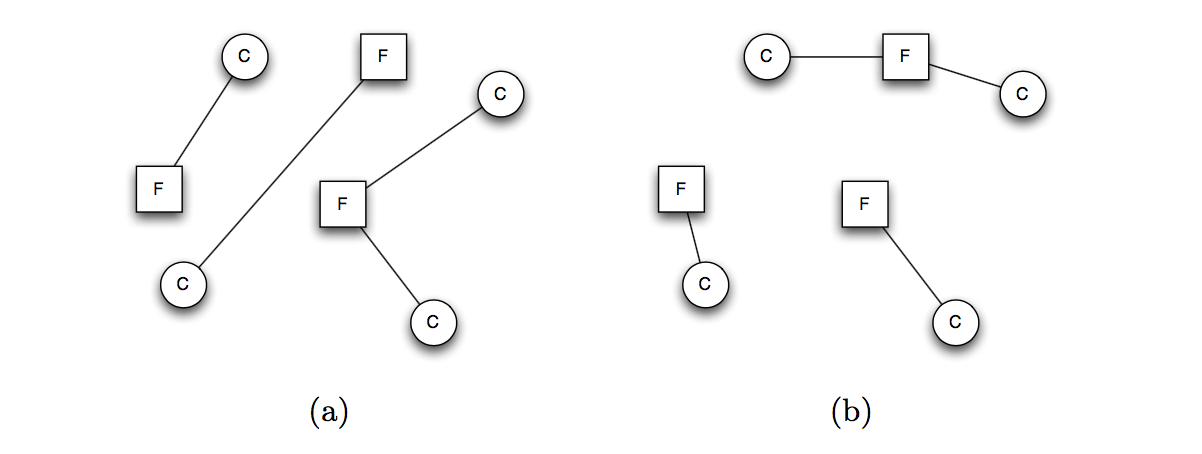
\includegraphics[width=150mm]{FLP}
    \caption{Lösung eines einfachen FLP}  \label{Typen}
  \end{center}
\end{figure}


Die beiden Beispiele besitzen jeweils drei Facilities (Depots) und vier Kunden (Nachfrageorte), wobei hier jeder Kunde nur von jeweils einer Basisstation beliefert wird, auch wenn wie bereits erwähnt andere Szenarien denkbar sind.
Wählt man nun die euklidischen Distanzen zwischen den Knotenpunkten als einzigen Kostenfaktor, ist es offensichtlich, dass Lösung b effizienter ist als a, da die Distanzen zwischen Depot und Kunden insgesamt geringer sind. 
Man spricht in diesem Fall von Verbindungskosten, wobei es allerdings ungenügend ist, sich nur auf die Verbindungskosten zu fokussieren, da in der Realität meistens noch Betriebskosten für Depots anfallen.
Zu diesen Betriebskosten zählen neben fixen Kosten, wie sie bei der Eröffnung einer neuen Basisstation entstehen würden, auch variable Kosten in Form von Personalkosten, die sich wiederum an den Öffnungszeiten der jeweiligen Basisstationen orientieren.

Wie bereits erwähnt ist J die Menge der Versorgungseinrichtungen (Facilities), in diesem Fall also die Menge aller Depots. 
Mit dem Parameter C werden im Folgenden die Anzahl aller Kunden beschrieben. 
Des Weiteren besitzen die Depots nicht-negative Kostenfunktionen f, welche die Betriebskosten (fix und variabel) jedes Depots darstellen. 

Dementsprechend wird eine Lösung gesucht, in der die Kosten minimiert werden.\\

Die Zielfunktion lautet dann:

\begin{equation}
Min \Sigma_{i} f_{i}  + \Sigma_{i} \Sigma_{j} dc_{ij} \cdot \beta_{ij} \cdot y_{j}
\end{equation}
 
minimiert.
Zusätzlich werden dem Problem die Binärvariablen $\beta_{ij}$ und $\gamma_{j}$ hinzugefügt, die den Wert 0 oder 1 annehmen können. Ist $\beta_{ij}$ = 1, so wird dem Kunden j ein Depot i zugeordnet. 
Die Variable  $\gamma_{j}$ entscheidet darüber, ob ein Depot ausgewählt wird ($\gamma_{j}$ = 1) oder nicht ($\gamma_{j}$ = 0). 
Nachdem fixe Kosten $f_{i}$ durch variable Kosten ersetzt werden und die Kosten der Lieferwege durch einen einheitlichen Satz c ersetzt werden, um die Kostenfunktion zu Vergleichszwecken der aus dem GAMS-Modell anzupassen, entsteht dadurch eine modifizierte Zielfunktion, welche auch in den nachfolgenden Kapiteln Anwendung findet:


\begin{equation} \label{obj}
Min \Sigma_{j} (close_{j}-open_{j})\cdot cp \cdot \gamma_{j}  + \Sigma_{i}\Sigma_{j} d_{i} \cdot \beta_{ij} \cdot c
\end{equation}\\



Unter den Nebenbedingungen:

\begin{equation} \label{eq:test11}
\Sigma_{j} d_{ij}\cdot \beta_{ij} <= Cap_{j}\cdot \gamma_{j} \hspace{5mm} \text{für alle i}
\end{equation}

\begin{equation} \label{eq:test0}
\Sigma_{i} d_{ij} \cdot \beta_{ij} = d_{i} \hspace{5mm} \text{für alle j}
\end{equation}

\begin{equation} \label{eq:test1}
\Sigma_{i} \beta_{ij} = 1 \hspace{5mm} \text{für alle j}
\end{equation}

\begin{equation} 
\beta_{ij} \in \{0,1\}
\end{equation}

\begin{equation} \label{eq:test}
\gamma_{j} \in \{0,1\}
\end{equation}


Die variablen Kosten einer Basisstationseröffnung in Form von Personalkosten finden sich im ersten Term der Zielfunktion (\ref{obj}) wieder, bei der die konkrete Zeit in Minuten, die eine Basisstation geöffnet hat, mit dem Minutensatz der Personalkosten verrechnet werden.
In den Nebenbedingungen wird zudem aufgezeigt, dass die Kapazität einer Basisstation nicht überstrapaziert werden darf (\ref{eq:test11}), so wie dies im GAMS-Modell in Restriktion (10) durch die Ungleichung festgehalten wird.
Außerdem wird durch die weiteren Restriktionen festgehalten, dass zum einen der komplette Bedarf eines Kunden gedeckt (\ref{eq:test0}) und jeder Kunde genau einer Basisstation zugeordnet wird (\ref{eq:test1}).

Beim FLP handelt es sich um ein NP-Schweres Problem. 
Solche komplexen Optimierungsprobleme werden meist mit approximativen Algorithmen berechnet.
Durch das FLP gelingt es demnach, eine Teilmenge aus verfügbaren Depots zu ermitteln, die optimal wäre für das in dieser Arbeit vorliegende Problem. 

 


\subsubsection{Modifizierung des Algorithmus zur Lösung des FLP}


Da sich herausstellte, dass sich das FLP als eine geeignete Problemstellung erweist, dessen Lösungsalgorithmus sich auch für weitere Anwendungen in dieser Arbeit als nützlich erweisen könnte, wird im Folgenden versucht, diesen Ansatz weiter zu verfolgen und den Algorithmus aus Vergleichszwecken zu modifizieren.

Das Facility Location Problem ist üblicherweise darauf ausgerichtet, einzelne Kunden mit mehreren Standorten zu beliefern, wobei dies wie bereits beim GAMS-Modell auf lediglich eine Basisstation pro Kunde beschränkt wird.
Die Modifizierung des Algorithmus gelingt, indem der gemischt-ganzzahligen Modellformulierung eine binäre Variable $\beta_{ij}$ hinzugefügt wird, die die folgende Restriktion erfüllt:


\begin{equation}
\Sigma_{j} \beta_{ij} = 1 \hspace{5mm}\text{für alle i}
\end{equation}


Die der gemischt-ganzzahligen Modellformulierung hinzugefügte binäre Variable $\beta_{ij}$ bzw. deren Restriktion ist somit vergleichbar mit der Restriktion (9) aus dem GAMS-Modell.

Würde die Modizierung des Algorithmus mit der Implementierung von $\beta_{ij}$ außen vor gelassen werden, so würde dies im weiteren Verlauf bei der Tourenbestimmung durch den genetischen Algorithmus auch Berücksichtigung finden müssen, was zu einem erheblichen Aufwand führen könnte, sodass diese Erweiterung nachfolgend in einem gesonderten Abschnitt untersucht wird.
Besonders herausfordernd dabei könnten die zusätzlich zu übermittelnden Informationen sein, die aus der Lösung des FLP in den genetischen Algorithmus hineingegeben werden müssen.
Bevor jedoch die Informationen aus der Lösung des FLP in den Ablauf der Lösung des VRP mit einfließen, wird Letzteres zunächst anhand eines Beispiels mit lediglich einer Basisstation im nächsten Kapitel vorgestellt, um diesen dann in den darauf folgenden Kapiteln zu modifizieren.


\subsection{Lösung eines ERP-TW durch GA}

\subsubsection{Grundlagen zum genetischen Algorithmus}

Genetische Algorithmen wurden in Anlehnung an die von Charles Darwin beschriebene natürliche Selektion entwickelt. Es handelt sich um einen biologischen Mechanismus, mit der nach dem Motto „survival of the fittest“ aus einer alten Population eine neue Population entsteht. \footnote{Vgl. Masum (2011), S. 126.}
Der genetische Algorithmus gehört zu den methaheuristischen Algorithmen und bietet vor allem bei komplexen kombinatorischen Optimierungsproblemen (NP-hard) wie dem Job Shop Scheduling Problem oder dem Vehicle Routing Problem erfolgsversprechende Lösungen an. 
Dabei beschreibt der GA einen evolutionären Prozess, anhand dessen eine neue Population entsteht.
Um den evolutionären Prozess des Algorithmus starten zu können, benötigt man zunächst eine Anfangspopulation. 
Eine Population besteht aus Individuen, die auch als Chromosom bezeichnet werden und jedes für sich eine Lösung der Problemstellung darstellt.
Ist der evolutionäre Prozess abgeschlossen, wird anhand der genetischen Fitness für jedes der Individuen entschieden, ob es in die neue Generation aufgenommen oder eliminiert wird. 
Die Fitness wird anhand einer Fitnessfunktion berechnet und variiert von der zu lösenden Problemstellung.
Der evolutionäre Prozess setzt sich im Allgemeinen aus den genetischen Operatoren Selektion, Crossover und Mutation zusammen.\footnote{Vgl. Masum (2011), S. 126.}
 
Der Crossover bezeichnet einen Vorgang, in dem zwei Elternpaare der Anfangspopulation miteinander gekreuzt werden. 
Die Gene im Chromosom der Elternteile werden dabei systematisch neu zusammengesetzt und bilden ein neues Nachkommen für die nächste Generation.
Somit entstehen bei einer Kreuzung zwei neue Nachkommen, jeweils als komplettes Chromosom für die nächste Generation. 
Das resultierende Chromosom muss häufig bestimmte Regeln erfüllen, die dank der Flexibilität des Algorithmus problemlos in diesen aufgenommen werden können.
In der Regel wird der Crossover-Prozess für zwei Elternchromosomen jeweils zweimal durchgeführt, sodass die neue Population von $n$ auf $2\cdot n$ Individuen verdoppelt wird.


\begin{figure}[h!]
  \begin{center}
    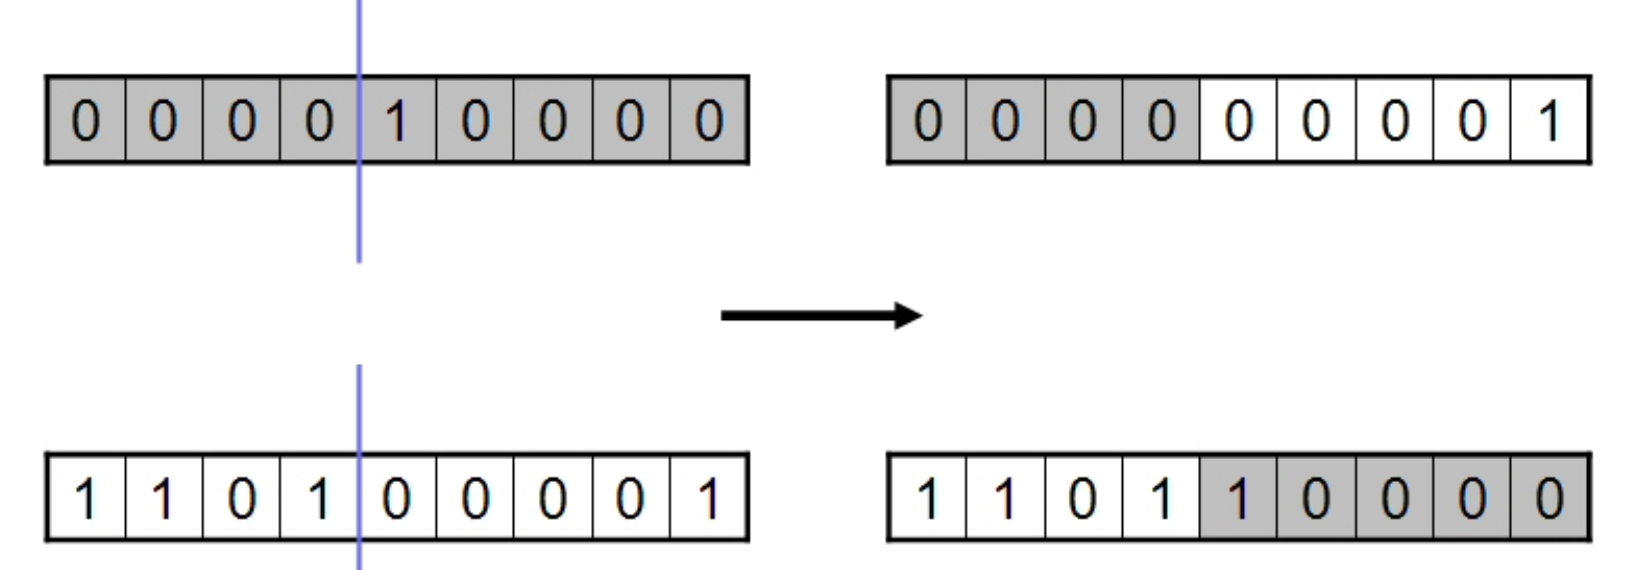
\includegraphics[width=100mm]{crossover.png}
    \caption{Crossover}  \label{Typen}
    {\footnotesize \textbf{Quelle:} Büning\footnote{Vgl. Büning, S. 11.}}
  \end{center}
\end{figure}


Die Kreuzung selbst kann durch eine Crossover-Wahrscheinlichkeit gesteuert werden. 
Bei einer Crossver-Wahrscheinlichkeit von 60\% werden bspw. durchschnittlich nur 6 von 10 aller Chromosome miteinander gekreuzt, wobei in der Praxis eine Wahrscheinlichkeit von mehr als 60\% als sinnvoll erwiesen ist\footnote{Vgl. Büning, S. 11.}, um möglichst viele neue Individuen entstehen zu lassen und so möglicherweise schneller konvergieren zu können.
Ist der Crossover-Prozess abgeschlossen, folgt die Mutation im genetischen Algorithmus.

Im Mutationprozess kommt es zu einer zufälligen Veränderung innerhalb eines Chromosoms. 
Dabei werden einzelne Gene innerhalb des Chromosoms vertauscht, wobei auch eine deterministisch festgelegte Mutations-Wahrscheinlichkeit eingehalten wird, sodass nicht jedes Chromosom mutiert wird. 
In der Regel wird dabei eine Wahrscheinlichkeit kleiner als 10\% gewählt.\footnote{Vgl. Büning, S. 15.}
Mit der Mutation wird versucht, die Population zu diversifizieren und neue Individuen, die weder durch den Crossover hervorgebracht wurden noch in der Anfangspopulation vorhanden waren, entstehen zu lassen. Vor allem bei größeren Populationen ist die Mutation durchaus sinnvoll, um Artenvielfalt zu gewährleisten. Sollte man nur den Crossover durchführen, läuft man stets Gefahr, bei einem lokalen Maximum hängen zu bleiben. Durch die Mutation besteht dann die Möglichkeit, von einem lokalen Maximum auf ein globales Maximum zu kommen. \footnote{Vgl. Goncalves et al. (2003), S. 82.}\\

Nachdem der Crossover und die Mutation beendet worden sind, erfolgt die Selektion der Individuen in die nächste Generation. 
Dabei ist es üblich, dass die besten Chromosome aus den ursprünglichen bzw. neu gebildeten Chromosomen in die neue Generation gelangen, wobei die restlichen Chromosome eliminiert werden. 
Es gibt jedoch verschiedene Verfahren bei der Auswahl der neuen Generation.
Im genetischen Algorithmus nach Goncalves gelangen bspw. alle neu gezeugten Individuen in die neue Generation ohne Rücksicht auf deren Fitness, wobei der Chromosomvorgang dort nur einmal pro Chromosompaar durchgeführt wird.\footnote{Vgl. Goncalves et al. (2003), S. 82.}

Des Weiteren kann die Auswahl der Individuen zufällig anhand einer Glücksrad-Strategie durchgeführt werden, wie sie im genetischen Algorithmus nach Berger und Barkaoui angewendet wird.\footnote{Vgl. Berger et al. (2003), S. 649.}
Dabei wird in einer Art und Weise vorgegangen, dass die neu erzeugten Individuen mit einer bestimmen Wahrscheinlichkeit proportional zu ihrer Fitness selektiert werden.\footnote{Vgl. Berger et al. (2003), S. 649.}


\paragraph{Darstellung der Chromosome}

Ein Chromosom setzt sich aus q Genen zusammen und wird in Vektorform repräsentiert. 
Die konkrete Ausprägung bzw. der Wert eines Gens wird dabei als Allel bezeichnet.
Dabei variiert die Bedeutung der Gene in den unterschiedlichen Problemstellungen. 
Im Job Shop Scheduling Problem können die Gene im Chromosom die Prioritäten und Verspätungszeiten von einzelnen Arbeitsschritten abbilden (Vgl. Goncalves et al., S. 82.), jedoch auch lediglich den Schedule, also die Reihenfolge der einzelnen Arbeitsschritte.
In Bezug auf das Vehicle Routing Problem stellen die einzelnen w Gene die zu beliefernden Kunden dar. 
Damit stellt ein gesamtes Chromosom eine mögliche Route eines Lieferroboters des VRP dar, wobei der Lieferroboter die Kunden in der Reihenfolge abfährt, wie es das Chromosom ihm vorschreibt. 


\subsubsection{Implementierung in Python}

Im Folgenden wird ein einfaches ERP-TW in Python implementiert, wobei es sich dabei um eine Lösung handelt, die auf einem genetischen Algorithmus basiert. 
Die Instanzen, die die Ausgangslage beschreiben, beinhalten dabei Information bezüglich geografischer Daten der Kunden und der einzelnen Basisstation sowie die gesamte Anzahl an Kunden, die von dieser einen Basisstation aus beliefert werden sollen.
Der Algorithmus ist zunächst sehr einfach gehalten, um den Hauptfokus auf die Erläuterung des genetischen Algorithmus zu legen. 
Im weiteren Verlauf dieser Arbeit wird dieser Algorithmus weiter modifiziert und stetig dem GAMS-Modell aus den vorherigen Abschnitten angepasst.

So analysiert der folgende Algorithmus im Gegensatz zu dem von Kleinschmidt (2017) die Ausgangslage mit lediglich einer einzigen Basisstation, von der aus die Fahrzeuge ihre Fahrt zu den einzelnen Kunden aufnehmen und zu der diese im Anschluss auch wieder zurückfahren, sodass die Standortbestimmung innerhalb des Algorithmus wegfällt.
Die maximale Kapazität der Basisstation ist zunächst unbeschränkt und stellt somit keinen eigenen Parameter dar, sodass Restriktion (10) aus dem GAMS-Modell entfällt. 
Auf zusätzliche Standortbestimmungen mittels Algorithmen zur Lösung des FLP wurde in dieser Arbeit bereits eingegangen, sodass der genetische Algorithmus im weiteren Verlauf so konzipiert werden muss, dass er die Informationen, die es aus der Lösung des FLP erhält, weiterverarbeiten kann.

Die Kapazitäten eines Akkumulators, sowohl hinsichtlich seiner geografischen als auch seiner zeitlichen Reichweite, werden berücksichtigt und können als Parameter selbst bestimmt werden (Restriktion 11, 12), sodass aus dem Modell wie zuvor im GAMS-Modell ein 'Electric Routing Problem with Time Windows' (ERP-TW) entsteht.\\

Ein Unterschied besteht auch in der Handhabung der Zeitfenster:

Werden diese im vorherigen Verfahren noch strikt eingehalten, können sie im Folgenden unter- bzw. überschritten werden, was allerdings zu Warte- bzw. Verspätungskosten führt und sich negativ auf die Fitnessfunktion auswirkt, je nach Gewichtung.
Dies dient lediglich der Vereinfachung des Problems, da sich im Folgenden wie bereits erwähnt gänzlich auf den genetischen Algorithmus und dessen Funktionsweise konzentriert werden soll. 
Feinheiten, die zu vergleichbaren Bedingungen führen, wie sie im GAMS-Modell vorliegen, werden in den nächsten Abschnitten vorgenommen. 

Die Geschwindigkeit des Fahrzeugs wird ebenfalls nicht als extra Parameter angegeben, sodass auch die Beachtung der Höchstgeschwindigkeit irrelevant wird.
Im Folgenden wird daher eine Distanzeinheit in exakt einer Zeiteinheit zurückgelegt, wodurch diese beiden Größen als gleichwertig anzusehen sind und in der Zielfunktion als eine Größe angesehen werden.
Die Personalkosten wurden nicht berücksichtigt, da lediglich eine Basisstation in Vollzeit geöffnet hat und somit diese Kosten bei allen möglichen Lösungen gleich wären, wohingegen Mietkosten für jeden verwendeten Lieferroboter erhoben werden, da es umso kostengünstiger ist, je weniger Lieferroboter verwendet werden.
Diese Mietkosten orientieren sich dabei am Parameter $flat$ des GAMS-Modells.

Begonnen wird mit der Ausrichtung aller vorhandenen Lieferroboter an den Koordinaten des Depots, welches den Startort für jegliche Lieferroboter darstellt.
In der Instanz wird das Depot als Kunde 0 dargestellt, um dem Algorithmus nicht zusätzliche Schwierigkeiten beim Einlesen der Informationen zu bereiten.
In einer Matrix werden jegliche Distanzen aller Kunden untereinander abgebildet, wobei sich diese Matrix an jener orientiert, die bereits in den Vorkapiteln in GAMS als Parameter verwendet wurde und im Anhang B eingesehen werden kann.
Jeder Kunde verfügt außerdem über Informationen bezüglich dem frühesten bzw. dem spätesten Zeitpunkt, in der er beliefert werden kann.
Diese beiden Informationen besitzt auch das Depot, wobei die Informationen hierbei dementsprechend aussagen, wann das Depot öffnet bzw. schließt.
Letztendlich enthält jeder Kunde eine weitere Angabe über die bei ihm vor Ort benötigte Servicezeit.

Zur Veranschaulichung wird im Folgenden ein Beispiel betrachtet, in welchem zwei Lieferroboter zehn Kunden so effizient wie möglich beliefern sollen.
Effizient insofern, sodass die gesamten Kosten, die sich aus Distanz- bzw. Zeitkosten (Warte- bzw. Verspätungszeit) zusammensetzen, so minimal wie möglich gehalten werden, wodurch auch die Zielfunktion des genetischen Algorithmus formuliert ist. 

Der genetische Algorithmus erstellt eine initiale Population aus einer vorgegebenen Anzahl an Chromosomen, die wiederum eine mögliche Lösung des ERP-TW darstellen. 
Ein Chromosom könnte demnach bei einer Anzahl von 10 Kunden folgendermaßen aussehen:

\begin{center}
[4, 3, 7, 9, 5, 2, 8, 6, 10, 1]

\end{center}

Dieses Chromosom besteht also aus 10 unterschiedlichen Genen, die jeweils einen Kunden darstellen, der beliefert werden soll.
 
Der erste Lieferroboter beginnt, den ersten Kunden im Chromosom, also hier Kunde 4, zu beliefern und geht das Chromosom so lange entlang, bis entweder die Kapazität des Lieferroboters erschöpft ist, die gesamte Zeit des Liefervorgangs die Schließzeit des Depots überschreitet oder die Akkukapazität hinsichtlich Reichweite bzw. Laufzeit ausgeschöpft ist, wobei im Detail folgendermaßen vorgegangen wird:\\
 
Zu Beginn wird Kunde 4 genauer untersucht, wobei zu diesem Zeitpunkt der Lieferroboters (theoretisch) keine Ladung aufgenommen und keine Zeit bzw. keine Distanz in Anspruch genommen hat.
Der Verbrauch des ersten Kunden mit dem Index 4 beträgt 1, wobei sich die Distanz zu diesem aus der euklidischen Distanz zwischen den Koordinaten des Depots und denen des Kunden berechnen (s. Anhang B).
Die Compartements eines Lieferroboters, also die gesamte Ladekapazität, wurde für das folgende Anwendungsbeispiel des genetischen Algorithmus auf 10 gesetzt, um dessen gesamtes Potential aufzuzeigen.

Nachdem die bisher verstrichene Zeit, die Dauer, die das Fahrzeug vom letzten Standort zum Kunden benötigt, die Dauer, die das Fahrzeug beim Kunden vor Ort verbringt sowie die Dauer, die das Fahrzeug vom Kunden zurück zum Depot benötigt aufsummiert wurden, wird diese Zeit mit der Schließungszeit des Depot verglichen (Restriktion (18)). 
Da die Summe der genannten Zeiten deutlich unter der Schließungszeit des Depots liegen und auch die Kapazität des Lieferroboters noch nicht voll ausgelastet ist, wird der Route dieses Lieferroboters der Kunde 4 hinzugefügt, da es möglich ist, ihn zu beliefern.

Nachdem dieses Prozedere für alle Gene im Chromosom vollzogen wurde, entsteht dabei folgende Aufteilung für die zwei verfügbaren Lieferroboter: 


\begin{equation} \label{eq:test}
    \begin{aligned} 
         Fahrzeug 1&: 0 - 4 - 3 - 7 - 9 - 5 - 2 - 0 \\
        Fahrzeug 2&: 0 - 8 - 6 - 10 - 1 - 0\\
    \end{aligned}
\end{equation}




Der Index 0 stellt hierbei das Depot dar, von dem das Fahrzeug zu Beginn startet und zu dem es am Ende wieder zurückfährt. Im Vergleich zu der Aufzählung der Touren für die einzelnen Fahrzeuge, bei der der erste Kunde den Index 1 zugewiesen bekommt, ist der erste Kunde auf der Karte mit dem Index 4 bezeichnet, sodass sich auch alle weiteren Kunden um drei Indizes nach rechts verschoben haben. 
Dies wird auch auf den in dieser Arbeit noch folgenden Abbildungen so gehandhabt.




\begin{figure}[h!]
  \begin{center}
    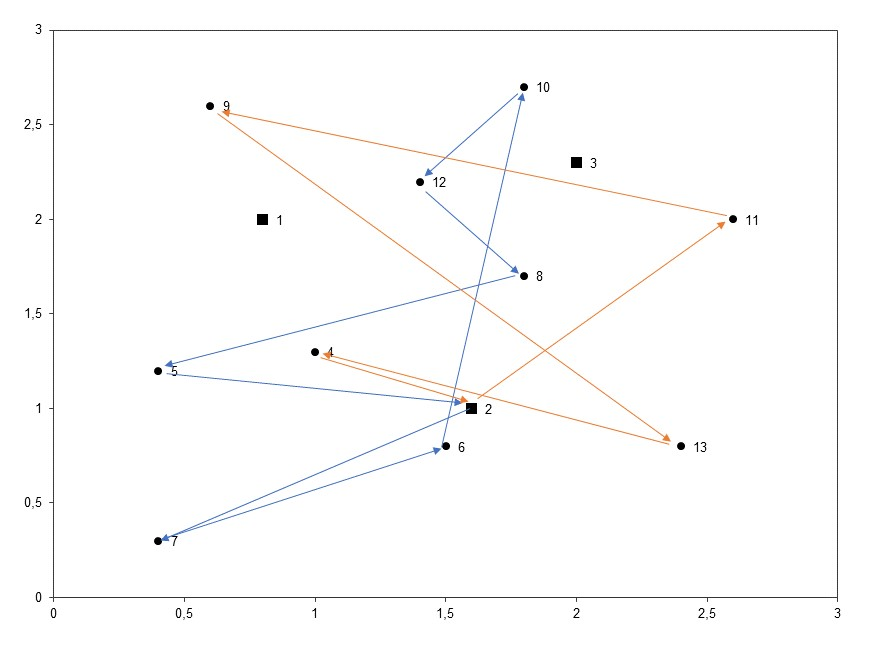
\includegraphics[width=100mm]{vrp11.jpg}
    \caption{Mögliche, solide Lösung des VRP}  \label{Typen}
    {\footnotesize \textbf{blau:} Fahrzeug 1;  \textbf{orange:} Fahrzeug 2}
  \end{center}
\end{figure}

Es werden somit alle 10 Gene des Chromosoms bzw. alle 10 Kunden durch die Tourenplanung abgedeckt, ohne dass dabei eine Restriktion gebrochen wird.
Um nun in Erfahrung zu bringen, wie effizient das vorliegende Chromosom ist in Bezug auf die Kosten, die es verursacht, wird im genetischen Algorithmus eine Evaluation durchgeführt, mit der die Fitnessfunktion berechnet wird. 
Nur anhand dieser Fitnessfunktion ist es dem genetischen Algorithmus möglich, effizient zu selektieren und sich iterativ weiterzuentwickeln.


\subsubsection{Evaluation des Chromosoms im genetischen Algorithmus}

Der Evaluationsprozess ist dafür zuständig, durch spezielle Methoden innerhalb des genetischen Algorithmus neuartige Chromosome innerhalb der Population zu bilden, sodass im Anschluss die Fitnessfunktion dieser berechnet werden kann und die Chromosome dadurch in der Population geordnet werden können, um somit die Selektion für die nächste Generation einzuleiten.
In dieser Evaluation werden zunächst die jeweiligen Routen der einzelnen Fahrzeuge auf deren Kosten untersucht, im Anschluss zusammengeführt, wobei diese Summe schließlich den Nenner der Fitnessfunktion bildet:

\begin{equation}
max F(x) = \frac{1}{tC}
\end{equation}

Kostenverursachende Faktoren sind hierbei lediglich die beiden Einheiten der Zeit- bzw. Distanz, welche beide als gleich kostenverursachend angesehen werden, sodass nur der Lieferweg sowie die Mietung eines neuen Roboters Kosten verursacht.

Das zuvor betrachtete Chromosom war das beste aus einer Anfangspopulation, die dadurch zustande gekommen ist, dass Chromosome zufällig zusammengewürfelt wurden.
Für jedes einzelne wurde im nächsten Schritt die Fitness berechnet, wobei das Chromosom [4, 3, 7, 9, 5, 2, 8, 6, 10, 1] mit dem Fitnesswert 0.0000002537 am besten abschnitt und somit näher durchleuchtet wurde.
Nun besteht jedoch die Möglichkeit, dass dies bei weitem nicht das beste Chromosom ist, da es lediglich das beste Chromosom aus der zufällig generierten Anfangspopulation ist, die aus 100 Chromosomen besteht, wobei die gesamte Anzahl an möglichen Chromosomen mit unterschiedlichen Anordnungen der Gene in der Anfangspopulation $9! = 362880$ beträgt.
Um herauszufinden, ob bessere Chromosome möglich sind, wurde in dieser Arbeit ein genetischer Algorithmus angewandt, für den bereits die Vorarbeit in Form der Generierung der Anfangspopulation geschaffen wurde.

\subsubsection{Crossover und Mutation}

Im nächsten Schritt wendet dieser Algorithmus in der ersten Iteration einen Crossover an, wodurch zwei zufällig gewählte Chromosome ausgewählt werden und auf eine zuvor festgelegte Art und Weise miteinander verknüpft werden, sodass am Ende zwei neue Chromosome entstehen, die wiederum in der Population mitaufgenommen werden.
Bei diesem Crossover kann es sich um die verschiedensten Methoden handeln, die jedoch stets auf Zufallsprozessen basieren.
Der genetische Algorithmus, der in dieser Arbeit Anwendung fand, schnitt dabei eine bestimmte Sequenz aus dem Chromosom, bspw. [5, 2, 8] und addierte diese mit der kompletten Sequenz eines weiteren Chromosoms, sodass diese drei Gene dem zweiten, anderen Chromosom voran standen und in der Sequenz nun doppelt vorkamen.\\
 
Die Doppelgänger, deren Pendant bereits schon einmal in der nun künstlich verlängerten Sequenz vorkamen, wurden gestrichen, sodass wiederum ein völlig neues Chromosom entstanden ist.
Dieser Vorgang wird für einen bestimmten Anteil der Chromosome vorgenommen, wobei dieser Anteil durch die vorher bestimmte Crossover-Wahrscheinlichkeit bestimmt wird. 
In dieser Arbeit konnten mit einer Crossover-Wahrscheinlichkeit i.H.v. 0.7 die besten Ergebnisse erzielt werden, sodass aus der Anfangspopulation von 100 Chromosomen ca. 70 Chromosome 35 Chromosompaare bildeten, die wiederum 70 neue Chromosome erschaffen haben, sodass im Anschluss der ersten Iteration eine neue Population mit insgesamt 170 Chromosomen entstanden ist. 
Aus diesen 170 Chromosomen werden nun abermals mit einem Zufallsprozess die 100 überdurchschnittlich besten (Glücksrad-Strategie) Chromosome mit in den nächsten Iterationsschritt mitaufgenommen, wobei darauf geachtet wird, dass mindestens der beste aus den 170 Chromosomen mit in diesen Schritt genommen wird, um die beste Lösung nicht zu verlieren und ggf. nicht noch einmal zu erhalten, was zum einen ein herber Verlust und zum anderen auch nicht im Sinne einer Optimierung wäre.



Bevor dieser finale Schritt innerhalb einer Iteration allerdings in die Wege geleitet wird, wird ein kleiner Bruchteil der Chromosome (hier: 1\%) nochmals mutiert, um zu gewährleisten, dass die Konvergenz des Algorithmus nicht zu früh eintritt und dieser sich u.U. in einem lokalen Minimum befindet. 
Auch hierbei existieren diverse Mutationsprozesse, die auf Zufallsmechanismen beruhen, wobei in dieser Arbeit auf einen Prozess zurückgegriffen wurde, der wiederum eine Sequenz des Chromosoms [5, 2, 8] herausschneidet und dieses an gleicher Stelle spiegelverkehrt [8, 2, 5] wieder einsetzt.\\

Nachdem 100 Iterationen mit einer Crossover- bzw. Mutations-Wahrscheinlichkeit i.H.v. 0.7 bzw. 0.01 bei einer Populationsgröße von 80 durchgeführt wurden, ergibt sich ein Chromosom, dass eine Fitness von 0.0005388 erreicht wird, was auch nach mehreren Durchläufen unerreicht bleibt und somit einen äußerst guten Wert darstellen sollte.
Das Chromosom nimmt dabei folgende Form an: 

\begin{center}
[10, 8, 7, 9, 4, 3, 2, 6, 5, 1]
\end{center}

und verteilt sich dabei wie folgt auf die drei zur Verfügung stehenden Fahrzeuge: 


\begin{equation} \label{eq:test}
    \begin{aligned} 
         Fahrzeug 1&: 0 - 10 - 8 - 7 - 9 - 4 - 3 - 0 \\
        Fahrzeug 2&: 0 - 2 - 6 - 5 - 1 - 0\\
    \end{aligned}
\end{equation}


\begin{figure}[h!]
  \begin{center}
    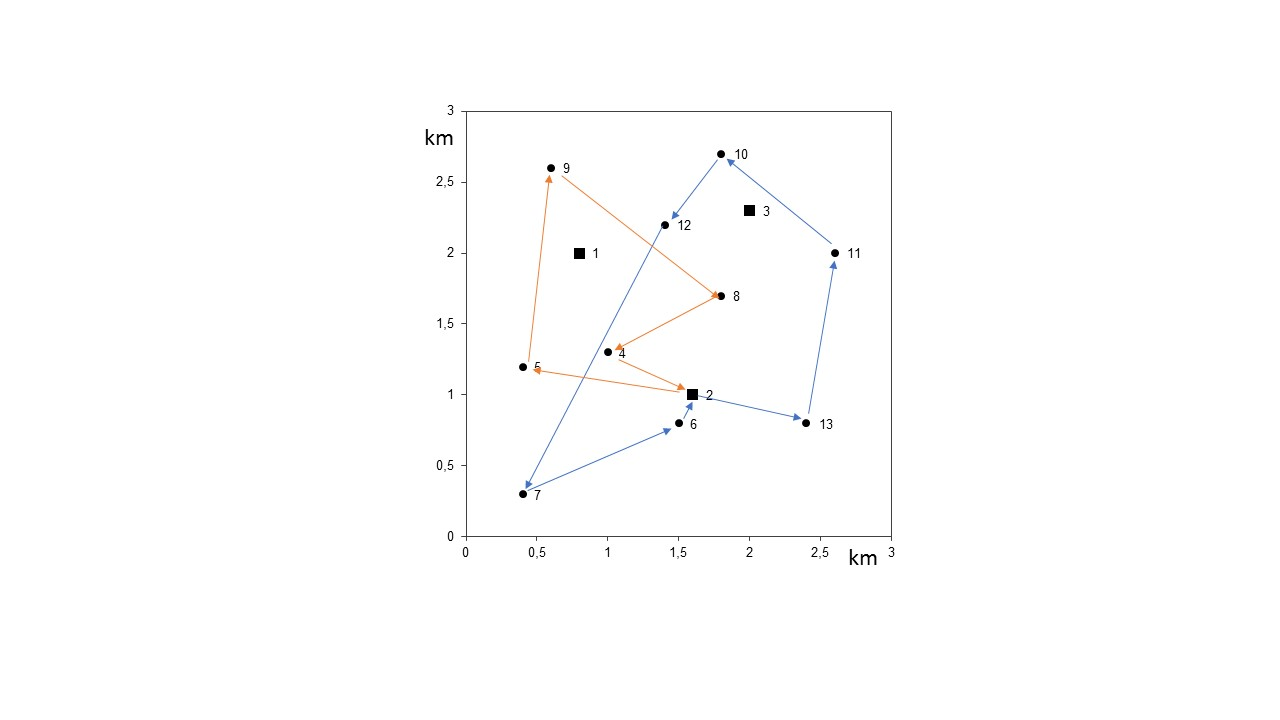
\includegraphics[width=100mm]{vrp222.jpg}
    \caption{Optimale Lösung des VRP}  \label{Typen}
	{\footnotesize \textbf{blau:} Fahrzeug 1, \textbf{orange:} Fahrzeug 2}
  \end{center}
\end{figure}


Auf Abbildung 4 kann diese Verteilung auf die Fahrzeuge eingesehen werden.\\

Nachdem das EVRP-TW erfolgreich mit einem genetischen Algorithmus analysiert und effizient gelöst werden konnte, wobei sich stets an die Angaben aus dem GAMS-Modell orientiert wurde, sowohl was die Informationen in der Instanz als auch die Parameter angeht, wird dieser Herangehensweise im folgenden Kapitel der Algorithmus vorangestellt, der zur Lösung des FLP angewandt wurde, um das resultierende Entscheidungsmodell mit dem GAMS-Modell vergleichbarer zu machen.


\subsection{Implementierung des Algorithmus zur Lösung des FLP in das ERP-TW}


Nachdem die optimalen Standorte mit dem modifizierten Facility Location Problem herausgefunden werden konnten, werden diese einzeln für sich mit dem Vehicle Routing Problem mittels genetischen Algorithmus konfrontiert.
Die Herausforderung dabei ist, dass es sich anstatt einer einzigen nun um mehrere Basisstationen handelt, deren Kunden so effizient wie möglich abgefahren werden sollen.
Die Kundenzuordnung wurde dabei bereits zuvor bei der Lösung des FLP ermittelt, sodass diese Information im nächsten Schritt dem genetischen Algorithmus übermittelt werden sollen, wodurch eine sequentielle Bearbeitung des Problems entsteht.

Die Zielfunktion orientiert sich dabei an der Zielfunktion im GAMS-Modell (1).
Öffnungs- bzw. Schließzeiten orientieren sich am GAMS-Modell und werden bereits in der Zielfunktion des FLP berücksichtigt.
Allerdings wird im genetischen Algorithmus nicht mit Zeitslots gearbeitet, so wie dies bei Kleinschmidt gehandhabt wurde.
Im genetischen Algorithmus entspricht hingegen eine Zeiteinheit genau einer Distanzeinheit und der Lieferroboter legt diese Distanzeinheit auch in genau einer Zeiteinheit zurück, sodass dies im Folgenden einer Modifikation bedarf, indem die Distanzeinheiten explizit durch die Geschwindigkeit geteilt wird, die dem Lieferroboter als Parameter gegeben wird.

Zu Vergleichszwecken wird dies dem GAMS-Modell insoweit angepasst, dass Angaben in Zeitslots mit dem Faktor 60 multipliziert werden, sodass im GA mit Zeiteinheiten in Minuten gerechnet wird. 
Auch wird für den Lieferroboter eine Durchschnittsgeschwindigkeit von 60 Meter pro Minute festgelegt, sodass alle Distanzeinheiten, die bei der Berechnung von Ankunftszeiten verwendet werden, durch diese Geschwindigkeit geteilt werden müssen(Gleichung (25)).
Die Entfernungen zwischen den Kunden bzw. Basisstationen werden in Metern angegeben.
Der Parameter $\alpha_{ghk}$, der den Wert 1 annimmt, wenn der Standort g vor dem Standort h auf der Route k angefahren wird, ist im genetischen Algorithmus nicht nötig, da die Routen durch die Chromosome genauestens definiert sind und lediglich abgefahren werden, sodass Restriktion (3) aus dem GAMS-Modell wegfällt.
So wird auch jeder Kunde nur einer Tour zugeordnet (Restriktion (2)), da jeder Kunde lediglich von einer Basisstation angefahren werden kann und von jener auch nur ein einziges Mal.

Aufgrund der festen Vorbestimmtheit der Touren durch das Chromosom und das Abfahren jenes wird zudem sichergestellt, dass jeder Standort auch jeweils einmal angefahren und verlassen wird, sich nicht selbst anfährt, keine Kurzzyklen entstehen und ein Ort auch nur innerhalb einer Tour angefahren werden kann, wenn er sich auf jener befindet (Restriktion (4,5,6)).
Die Kapazität des Fahrzeugs in Gestalt von Compartements ist auch bereits im Algorithmus integriert und wird bei der Planung der Routen berücksichtigt.
Bei Betrachtung der einzelnen Basisstationen wird auch eine Variable zur Kapazitätsbeschränkung jener eingeführt, wobei diese sich wiederum an der Variable $Cap_{j}$ aus dem GAMS-Modell orientiert.\\

Um die Problematik auf ein Problem mit elektrischer Komponente zu erweitern, wurde bereits im genetischen Algorithmus eine Akkukomponente eingeführt, bei der lediglich Zeit- und Distanzeinheiten angepasst werden.
Konnten die Zeitfenster im genetischen Algorithmus in dessen Vorstellung noch unter- bzw. überschritten werden, was mit erheblichen Kosten verbunden war, so ist dies in der Implementierung des FLP in den genetischen Algorithmus aus Vergleichszwecken nicht mehr gestattet. 
Da es jedoch sinnvoll sein könnte, diese Zeitfenster nicht immer einzuhalten und bewusste Verzögerungen mit einfließen zu lassen, werden diese Über- bzw. Unterschreitungen im nachfolgenden Abschnitt als Erweiterung des Modell diskutiert.
Das Modell, das nun durch den Algorithmus zur Lösung des FLP ergänzt wird, arbeitet somit ebenfalls mit Zeitbeschränkungen, so wie dies auch schon beim GAMS-Modell der Fall war, wobei sich an den Öffnungs- bzw. Schließungszeitpunkten der Zeitfenster der jeweiligen Kunden orientiert wird, die auch schon in diesem Modell verwendet wurden.

Binärvariablen, wie sie im GAMS-Modell bzw. im Algorithmus zur Lösung des FLP vorkommen, sind bei der Lösung des VRP durch den GA nicht vorgesehen.
Eine besondere Herausforderung bei der Implementierung besteht darin, dem genetischen Algorithmus die Kunden und ihre dazugehörigen Basisstationen, die durch die vorherige Standortbestimmung ermittelt wurden, zu übermitteln.
Dafür wird diese Information der Stationszuweisung direkt im Anschluss an die Lösung des FLP in die Instanz implementiert, die dann wiederum vom genetischen Algorithmus abgerufen wird.
Nur auf Basis dieser Information ist es dem GA möglich, eine gesonderte Betrachtung für jede einzelne Basisstation durchzuführen.
Jene Betrachtung wird durchgeführt, indem die Instanz in drei verschiedene Instanzen aufgeteilt wird, wobei jede Instanz für sich die Informationen über Kunden und Fahrzeuge enthält, die für die jeweilige Basisstation von Bedeutung sind.
Nur so kann der genetische Algorithmus explizit die Basisstationen gesondert untersuchen und deren optimale Touren vereinzelt planen. 
Nachdem der genetische Algorithmus die separate Instanz aufgenommen hat, baut er wiederum eine Anfangspopulation aus einer bestimmten Anzahl an Chromosomen, die wiederum exakt so viele Gene in sich beinhalten wie Kunden derjenigen Basisstation zugeordnet sind, deren Instanz untersucht wird.

Bei der Routenplanung wird dann das zufällig generierte Chromosom abgelaufen und die Gene solange einer Route zugeordnet, bis eines der Beschränkungen nicht eingehalten wird, wobei dies folgende sind:
 
Zum einen muss die Akkukapazität sowohl bzgl. seiner Laufzeit als auch seiner Reichweite vom Kunden, dessen Hinzunahme zur Route im aktuellen Schritt überprüft wird, zum Depot reichen. 
Ist dies nicht der Fall, bricht der Algorithmus an dieser Stelle ab und verweist den Kunden auf eine neue Tour.
Der Puffer, den der Akku dabei im GAMS-Modell sowohl hinsichtlich seiner Laufzeit als auch seiner Reichweite bekommen hat, wird im Algorithmus nicht extra erwähnt sondern direkt von der Akkulaufzeit bzw. -reichweite abgezogen, was lediglich der Übersichtlichkeit der Codierung dienlich ist.

Auch die Ladekapazität des Fahrzeugs muss für diesen zusätzlichen Kunden ausreichen (Restriktion (7)), wobei sich diese dabei am Parameter $Comp$ aus dem GAMS-Modell orientiert, der die Compartements eines Fahrzeugs angibt, welche in der gleichen Einheit angegeben werden wie auch schon die Nachfrage der einzelnen Kunden.
Bereits im FLP wurde eine Restriktion eingeführt, sodass gewährleistet wird, dass alle Kunden auch ausreichend versorgt werden von den kapazitätsbeschränkten Basisstationen.
Zuletzt kann der Kunde auch nur dann mit in die aktuelle Tour aufgenommen werden, wenn bei der Ankunftszeit das Zeitfenster eingehalten wird, das dieser Kunde bei seiner Bestellung angegeben hat.
Dabei muss nicht nur die Fahrzeit, die das Fahrzeug vom Kunden, bei dem es momentan anwesend ist, sondern auch die Service-Zeit, in der das Fahrzeug beim Kunden verweilt, berücksichtigt werden.


\subsection{Diskussion der Ergebnisse}

Die im vorherigen Abschnitt vorgestellte Herangehensweise stellt einen kombinierten Ansatz an die Problemstellung der Nutzung elektrisch betriebener Lieferroboter in der urbanen Logistik dar, wobei sich diese Herangehensweise aus der sequentiellen Bearbeitung des FLP und des ERP-TW zusammensetzt.

Das vorangegangene FLP wurde dabei mit der Pythonversion 3.6.3 berechnet, welches sich einer Optimierungssuite bediente, die auf ein Branch-and-Bound-and-Price Verfahren zurückgriff, wobei der Solver SCIP\footnote{Siehe hierzu http://scip.zib.de.} für eine gemischt-ganzzahlige Modellformulierung dieses Verfahren angewandt hatte.
Ziel des Algorithmus zur Lösung des FLP war es, dieses mit minimalen Kosten im Hinblick auf kostenverursachende Lieferwege effizient zu lösen.


Im Algorithmus zur Lösung des FLP verhält es sich bei der Deklarierung der Variablen ähnlich zu dem im GAMS-Modell, sodass auch in der Syntax von Python Variablen entweder als 'binär' oder als 'Integers' einzustufen sind.
Die Ergebnisse, die daraufhin im genetischen Algorithmus zustande gekommen sind, wurden ebenfalls mithilfe des Analysetools Python in der Version 3.6.3 berechnet, da dies einer leichteren Implementierung der Ergebnisse aus dem FLP dienlich war.
Die Leistung des dabei zum Einsatz gekommenen Rechners (Windows 10, 64-Bit, Intel Core i5 8250U) ist bei 1.60GHz mit 4 Kernen und einem Arbeitsspeicher von 8GB einzustufen, sodass es Sinn ergeben könnte, Abbruchkriterien in den Algorithmus mit aufzunehmen.
Wurde auf dieses noch im FLP verzichtet, so wurde beim genetischen Algorithmus ein Abbruchkriterium i.H.v. von 100 Iterationsschritten eingeführt.
Einschränkungen der Variablen im FLP wurden dabei nicht vorgenommen.\\

Der betrachtete Anwendungsfall bezieht sich wie bei bereits im GAMS-Modell auf ein Stadtgebiet mit 13 fiktiven Orten, 3 für die Basisstationen und die restlichen 10 für die Kunden, wobei die Lage der Orte auf Abbildung 5 entnommen werden kann.
Auch entspricht die Entfernung zwischen den Orten der euklidischen Distanz zwischen den x- bzw. y-Koordinaten, die in der Instanz zur Verfügung gestellt werden.

Eine Ermittlung der Lösung kam bereits nach 1,27753 Sekunden zustande, wobei durch diese Gesamtkosten i.H.v. 825,491 Einheiten aufkommen.
Durch das vorangegangene FLP wurden Basisstationen an den Orten 2 und 3 eröffnet, wovon allerdings insgesamt 7 Touren durch den genetischen Algorithmus als die optimale Tourenanzahl ermittelt wurden.
Veranschaulicht werden diese Routen in der folgenden Abbildung, wobei sogleich auffällt, dass die beste Lösung des metaheuristischen Verfahrens aus vielen Einzelteilen besteht.  



\begin{table}[h!]
    \vspace*{-3mm}
    \hspace*{2mm}
  \renewcommand{\arraystretch}{1,5}
  \caption{Lösungen der sequentiellen Herangehensweise
  }
  \begin{center}
 
    \begin{tabular}{|l|l|l|l|} \hline
    \textbf{Gesamtkosten (GE)} &\textbf{BS} &\textbf{Anzahl Touren}&\textbf{ Rechenzeit} (Sek)\\\hline
     825,491 & 2;3 & 7 & 1,27753\\\hline   
	\end{tabular}
	  \end{center}
\end{table}


Die Routen der vier Touren der zweiten Basisstation sind folgende: 

\begin{equation} \label{eq:test}
    \begin{aligned} 
         Fahrzeug 1&: 0 - 5 - 6 - 0 \\
        Fahrzeug 2&: 0 - 13 - 0\\
        Fahrzeug 3&: 0 - 4 - 7 - 0\\
        Fahrzeug 2&: 0 - 8 - 0\\
    \end{aligned}
\end{equation}\\

Die Routen der drei Touren der dritten Basisstation sind folgende: 

\begin{equation} \label{eq:test}
    \begin{aligned} 
         Fahrzeug 1&: 0 - 9 - 0 \\
        Fahrzeug 2&: 0 - 11 - 12 - 0\\
         Fahrzeug 3&: 0 - 10 - 0\\
    \end{aligned}
\end{equation}



\begin{figure}[h!]
  \begin{center}
      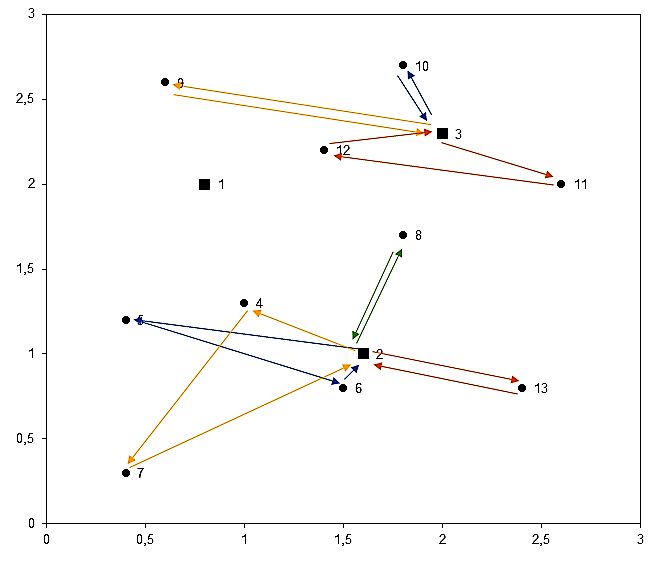
\includegraphics[width=100mm]{vrp33a.png}
    \caption{Lösung mit genetischem Algorithmus}  \label{Typen}
  \end{center}
\end{figure}


\begin{figure}[h!]
  \begin{center}
    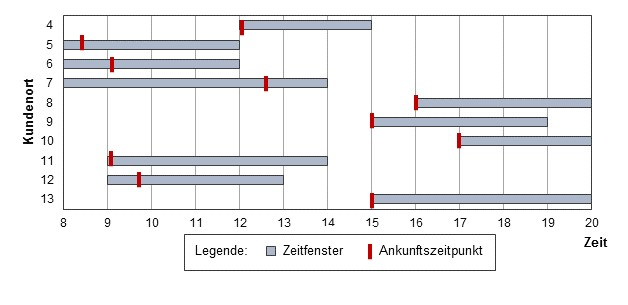
\includegraphics[width=150mm]{zf1.jpg}
    \caption{Zeitfenster für die Lösung mit GA}  \label{Typen}
  \end{center}
\end{figure}


Es ist auffällig, dass die sequentielle Bearbeitung der Problemstellung mit deutlich schnelleren Bearbeitungszeiten einhergeht, jedoch die Lösung wiederum zu zerstückelt ist, sodass hier ein Zusammenhang bestehen könnte.

Obwohl sie durch einen deutlich schwächeren Prozessor (1.6GHz statt 2.5GHz) ausgeführt wurden, entsprachen die Bearbeitungszeiten der zweiten Herangehensweise nur einem Bruchteil derjenigen, die das GAMS-Modell mit einer nichtlinearen Modellkonstellation benötigte und kam dabei nur auf marginal schlechtere Ergebnisse.
Auch bei Umformulierung der Parameter und der damit erzeugten Linearisierung des Modells war das sequentielle Modell ca. doppelt so schnell wie das GAMS-Modell.
Bei starker Ähnlichkeit der Ergebnisse könnte man demnach berechtigterweise zu dem Schluss kommen, dass es sinnvoller wäre, im Hinblick auf die Bearbeitungszeit anstatt des GAMS-Modells einen Algorithmus zu verwenden, der sich nur zu einem Teil auf einen optimierenden Solver stützt, einen anderen Teil jedoch in ein metaheuristisches Verfahren durch die Untersuchung des EVRP-TW mit einem genetischen Algorithmus ausgegliedert hat.\\

Bei näherer Betrachtung der Ergebnisse war jedoch der Grund hierfür direkt auszumachen: das sequentielle Modell optimierte nicht die Startzeitpunkte, in der ein Lieferroboter die Basisstation verlässt und sich auf die Reise zum ersten Kunden der ihm zugewiesenen Tour macht, sodass der erste Kunde einer Tour stets zum frühesten Zeitpunkt angetroffen wird.
Dies stellte insofern einen Nachteil dar, da bei bewusster Verzögerung des Starts eines Lieferroboters Kunden unter Umständen noch mit auf die Tour aufgenommen werden könnten, sodass hier an Effizienz eingebüßt wurde, welche sich auch in den unterschiedlichen Gesamtkosten direkt bemerkbar machten. 
IM GAMS-Modell wird der erste Kunde einer Tour, Kunde 6, erst sehr spät angefahren, wie Abbildung 3 entnommen werden kann, sodass es möglich ist, auch den Kunden 4 noch mit auf die Tour zu nehmen, dessen Zeitfenster sich erst um 12 Uhr öffnet. 
Im genetischen Algorithmus hingegen wäre der Kunde 6 bereits zum frühesten Zeitpunkt, hier um 8:04 Uhr, angefahren worden, sodass der Kunde 4 nicht mehr mit auf die Tour mitgenommen wird (Abbildung 6), worunter die Effizienz der Tour leidet und es zu erwähnter Zerstückelung kommt.
Der erste Lieferroboter mit der leeren Tour wurde im Anschluss an die Touroptimierung zwar gelöscht, sodass keinerlei Kosten in Form von einer Mietkostenpauschale entstanden ist, jedoch wäre eine direktere Anweisung seiner Startzeit nicht nur wünschenswert sondern vor allem auch unter Umständen kostensparender gewesen.\\

Die Bearbeitungszeit der hier vorliegenden Arbeit war leider zu kurz, um dem genetischen Algorithmus, der \textit{from scratch} (engl.: 'fast aus dem Nichts') erschaffen wurde, diese zusätzlichen Fähigkeit der Startzeitbestimmung einzuimpfen, sodass hier ein großer Raum für weitere Nachforschungen geschaffen wurde, gerade im Hinblick auf faire Vergleiche mit dem GAMS-Modell.
Diese Problematik des GA schlägt sich dann dementsprechend direkt auf die Bearbeitungszeit nieder, sodass an dieser Stelle von einem nicht-fairen Vergleich der beiden Herangehensweisen hinsichtlich ihrer Bearbeitungszeiten gesprochen werden muss.

Aufgrund dieser Umstände ist es in den Lösungen des sequentiellen Modells dazu gekommen, dass es zu viel mehr Touren kam als im simultanen GAMS-Modell (7 statt 4), sodass ein Ziel, nämlich die Vermeidung von zu vielen Touren, im zweiten Modell deutlich verfehlt wurde.
Auffällig war, dass der dem EVRP vorangegangene Algorithmus zur Lösung des FLP die gleichen Ergebnisse hinsichtlich der optimalen Standpunkte der Basisstationen hervorbrachte, wie dies auch schon im simultanen GAMS-Modell geschah. 
Da die Lösungen, die durch den GA zustande gekommen sind, sehr zerstückelt und für die Praxis nahezu unbrauchbar sind, legt dies nur die Vermutung nahe, dass die simultane Herangehensweise die zwar etwas langsamere, aber doch effizientere Lösung für den operativen Einsatz zu sein scheint, wie dies auch schon an den geringeren Kosten deutlich wird.	
Insgesamt stellt sich die Frage, ob bei einer solch kleinen Ausgangsinstanz eine heuristische Herangehensweise sinnvoll ist.


Kritisch zu hinterfragen sind außerdem die Einschränkungen, die dem in den vorangegangen Kapiteln vorgestellten Modell durch Kleinschmidt auferlegt wurden. 
So ist es zum einen für die Berechnungen zwar durchaus sinnvoll, jedem Kundenort lediglich eine Basisstation zuzuordnen, da dadurch die Komplexität der Problemstellung stark abnimmt. 
Allerdings ist es durchaus sinnvoll im Hinblick auf die Senkung der Gesamtkosten, dass ein Kunde von mehreren Basisstationen beliefert werden könnte, sodass sich dieser Idee in den Erweiterungen des Modells im anschließenden Kapitel gewidmet wird.
Zusätzlich zu der Erweiterung des Modells durch das Zulassen der Belieferung von Kunden durch mehrere Basisstationen erscheint eine weitere Zulassung sinnvoll: die Nichteinhaltung der Zeitfenster mit sich auf die Kostenfunktion negativ auswirkenden Kosten.


\newpage

\section{Erweiterungen}

\subsection{Zulassen von mehreren Belieferungen je Kundenort}

Aufgrund der stark eingeschränkten Kapazität des Fahrzeugs muss eine Tour häufig bereits nach wenigen Kunden abgebrochen werden, sodass es eine sinnvolle Erweiterung des Modells wäre, wenn jeder Kunde zusätzlich von weiteren Robotern, die sich auf anderen Touren befinden, beliefert werden könnte.
Ein Kunde mit einer Nachfrage von $d_{i} = 1$ könnte dann von einem Lieferroboter beliefert werden, der noch ein Compartement frei hätte auf seiner bereits bestehenden Tour, sein nächster Kunde jedoch 2 Compartements für sich in Anspruch nehmen würde.
Dabei muss bereits in den Algorithmus zur Lösung des dem EVRP vorangegangenen  FLP eingegriffen werden, wobei Restriktion (\ref{eq:test1}) aus dem Modell entfernt wird, um so zu gewährleisten, dass bereits im FLP jedem Kunden mehr als eine Basisstation zugeordnet werden kann.
Diese Information muss dann der Instanz, die nach dem Teilen der Gesamtinstanz für eine Basisstation übrig bleibt, zusätzlich hinzugefügt werden, ehe der genetische Algorithmus auf die Teilinstanz als Ausgangspunkt für seine Berechnungen zurückgreift.





%
%
%\subsection{Belieferungen der Kundenorte außerhalb des Zeitfensters}
%
%Da das Niveau des Kundenservices zu den wesentlichen Einflussgrößen hinsichtlich Kosten gehört, sollte es eigentlich außer Frage stehen, dass der Kunde auch in seinem Zeitfenster beliefert wird.
%Sollte es sich allerdings nur um kurze Verspätungs- bzw. Wartezeiten des Fahrzeugs beim Kunden handeln, sodass dieser dafür mit auf eine bereits bestehende Tour genommen werden kann, könnte es durchaus sinnvoll sein, dieses Zeitfenster mit vorheriger Benachrichtigung und einem Einverständnis des Kunden zu über- bzw. unterschreiten.
%Diese Warte- bzw. Verzögerungszeiten würden sich dann wiederum auch negativ auf die Kosten einer Tour auswirken, wobei diese Kosten dann eher immaterieller Natur wären in Form von Imageschäden. 
%Abgewogen sollte in diesem Zusammenhang auch die Frage, wie hoch diese Kosten in Relation zu anderen Kosten sein sollten.
%
%Es würde so allerdings gelingen, den Kunden 4 sowie den Kunden 7, die beide zur Basisstation 2 zugehörig sind, mit auf die erste Tour zu nehmen und so eine Neuinitialisierung eines Lieferroboters speziell für diese beiden Kunden aus dem Weg zu gehen.
%



\subsection{Diskussion der erweiterten Modelle}

Nach einer Vielzahl an Untersuchungen nach Änderungen der Variable c konnte es nicht gelingen, durch den Algorithmus zur Lösung des FLP ein Resultat zu erhalten, welches einen Kunden zu zwei Basisstationen zuwies.
So besteht hier ein deutlicher Unterschied zu der Lösung, die durch das erweiterte GAMS-Modell gefunden wurde, als die Restriktion, die einem Kunden stets eine Basisstation zugewiesen hat, aufgehoben wurde.
Erst nachdem die Nachfrage $d_{i}$ des Kunden 8 auf den Wert 15 hochgesetzt wird, wobei alle weiteren Variablen ceteris paribus gleich bleiben, gelangt man für diesen Kunden durch den Algorithmus zu einer Lösung, die diesen Kunden zu den Basisstationen zwei und drei zuweist.
Dabei erhält Kunde 8 aus der Basisstation zwei drei Einheiten und aus Basisstation drei 12 Einheiten, sodass auch die Ladekapazität des Lieferroboters auf 12 Einheiten hochgesetzt wird.


\begin{table}[h!]
    \vspace*{-3mm}
    \hspace*{2mm}
  \renewcommand{\arraystretch}{1,5}
  \caption{Lösungen der sequentiellen Herangehensweise
  }
  \begin{center}
 
    \begin{tabular}{|l|l|l|l|} \hline
    \textbf{Gesamtkosten (GE)} &\textbf{BS} &\textbf{Anzahl Touren}&\textbf{ Rechenzeit} (Sek)\\\hline
     925,659 & 2;3 & 8 & 1,4890\\\hline   
	\end{tabular}
	  \end{center}
\end{table}


Die Routen der vier Touren der zweiten Basisstation sind folgende: 

\begin{equation} \label{eq:test}
    \begin{aligned} 
         Fahrzeug 1&: 0 - 8 - 0 \\
        Fahrzeug 2&: 0 - 13 - 0\\
        Fahrzeug 3&: 0 - 6 - 5 - 0\\
        Fahrzeug 2&: 0 - 1 - 4 - 0\\
    \end{aligned}
\end{equation}\\

Die Routen der drei Touren der dritten Basisstation sind folgende: 

\begin{equation} \label{eq:test}
    \begin{aligned} 
         Fahrzeug 1&: 0 - 9 - 0 \\
        Fahrzeug 2&: 0 - 8 - 0\\
         Fahrzeug 3&: 0 - 10 - 0\\
         Fahrzeug 4&: 0 - 11 - 12 - 0\\
    \end{aligned}
\end{equation}


Auffällig ist zum einen, dass die Bearbeitungszeit marginal länger ist im Vergleich zu der aus dem vorherigen Modell. 
Zum anderen wird deutlich, dass nun 8 Lieferroboter anstatt 7 durch den Algorithmus zur Lösung des VRP den Kunden zugewiesen werden, was lediglich darauf zurückzuführen ist, dass der 8. Kunde nun auch von der Basisstation 3 beliefert werden kann.
Es hat demnach keinerlei Auswirkungen auf das Ergebnis, wie hoch die maximale Kapazität der Basistationen (hochgesetzt auf 20) bzw. der Lieferroboter (hochgesetzt auf 12) sind, was für eine weiterführende Sensitivitätsanalyse von großer Bedeutung ist, da diese im GAMS-Modell noch zu anderen Ergebnissen bzgl. des Parameters $Comp$ gelangte.
Eine ausführliche Sensitivitätsanalyse würde in dieser metaheuristischen Herangehensweise jedoch den Rahmen sprengen, wäre allerdings für weitere Nachforschungen von großer Relevanz.\\


\begin{figure}[h!]
  \begin{center}
      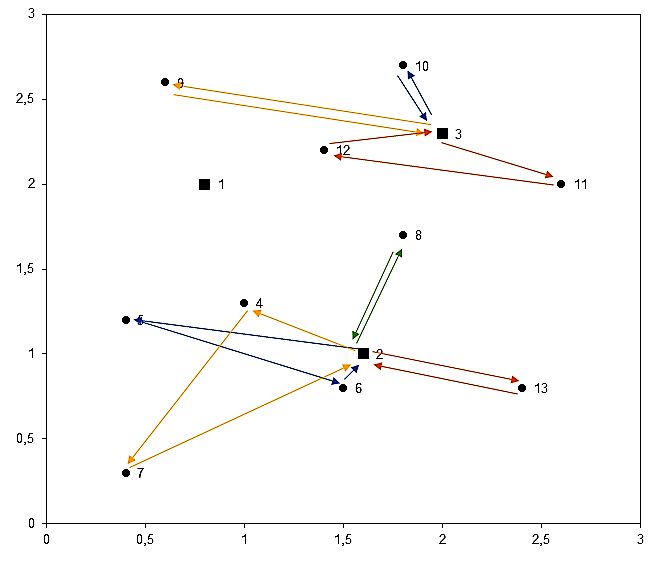
\includegraphics[width=100mm]{vrp33a.png}
    \caption{Lösung mit genetischem Algorithmus}  \label{Typen}
  \end{center}
\end{figure}


\begin{figure}[h!]
  \begin{center}
    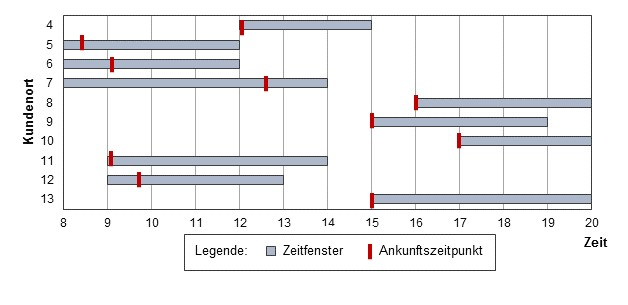
\includegraphics[width=150mm]{zf1.jpg}
    \caption{Zeitfenster für die Lösung mit GA}  \label{Typen}
  \end{center}
\end{figure}



Abschließend ist noch zu erwähnen, dass der Algorithmus in der kurzen Bearbeitungszeit lediglich so weit entwickelt werden konnte, dass er Informationen im Fall von zwei verschiedenen Basisstationen, die sich auf einen Kunden beziehen, weitergeben kann.
Für den Fall, dass die Auflösung des FLP ergibt, dass ein Kunde von drei verschiedenen Basisstationen beliefert wird, übermittelt der Algorithmus eine Fehlermeldung.
Somit ist hier viel Raum für Nachforschungen entstanden, um den Algorithmus auf eine allgemeine Problemstellung anwenden zu können, gerade im Hinblick darauf, dass ein metaheuristisches Verfahren wie es der genetische Algorithmus darstellt erst ab einer bestimmten Instanzgröße sein volles Potential zum Ausdruck bringen kann.



\newpage
%\section{Limitationen und Handlungsempfehlungen}


%Im Folgenden wird zunächst untersucht, welchen Limitationen bei der Bearbeitung der Problemstellung gegenübergetreten werden musste. 
%Eine Schwierigkeit bei der Implementierung des genetischen Algorithmus in Python stellte dabei vor allem die Angelegenheit dar, dem Lieferroboter seine genaue Startzeit am Depot mitzuteilen. 
%So startete dieser, wenn das Depot eröffnete in der Hoffnung, den ersten Kunden im Chromosom auch in seinem Zeitfenster zu erreichen. 
%Gelang dies nicht, so wurde der Kunde direkt einer neuen Tour mit einem neuen Lieferroboter zugewiesen. 
%Falls dies geschieht, so startet der neue Lieferroboter exakt zu dem Zeitpunkt an der Basisstation, sodass er genau pünktlich zum Beginn des Lieferfensters am Standort des ihm neu zugewiesenen Kunden ankommt.
%Dadurch kommt es vor, dass der Lieferrobotern bei späteren Kunden vor Beginn des Zeitfensters ankommt, obwohl es im Bereich des Möglichen gewesen wäre, bei einer späteren Ankunft beim ersten Kunden diesen späteren Kunden noch mitzunehmen.
%Bspw. geschieht dies im GAMS-Modell, wie der Abbildung 3 zu entnehmen ist. 

%
%
%Anschließend an die eben beschriebenen Limitationen werden im Folgenden Handlungsempfehlungen dargelegt, durch die potentielle Verbesserungen des Modells in die Wege geleitet werden könnten.
%Da es wie in der Diskussion zum GAMS-Modell bereits angesprochen sinnvoll erschien, dass Tourenproblem nicht ebenfalls simultan zum Standortproblem ablaufen zu lassen, da letzteres einer gewissen Schnelllebigkeit ausgesetzt ist aufgrund der täglich variierenden Kundenstandorte.
%Macht man nun das Standortproblem von der Tourenplanung abhängig, so wie dies im GAMS-Modell geschehen ist, so könnte eine optimale Lösung am nächsten Tag bereits wieder suboptimal bzw. schlecht sein.
%Um dieser Angelegenheit etwas entgegenzusetzen, wäre es in einem fiktiven Fall möglich, dass man die optimalen Standorte nicht aus einer Menge an bereits geografisch feststehenden Standorten wählen muss, sondern eine gesamte Menge an potentiellen Kunden durch Clustermethoden zunächst zu clustern und diesen im gleichen Zuge ein Zentrum zuweisen würde, welches dann die Basisstation für die zu diesem Cluster zugewiesenen Kunden bildet.
%Die Kunden könnten dabei eine gewisse Wahrscheinlichkeit zugewiesen bekommen, die sich darauf bezieht, wie wahrscheinlich es ist, dass diese Kunden in naher Zukunft zu den Kunden gehören.
%Diese könnten dann wiederum durch zweidimensionale Wahrscheinlichkeitsverteilungen wie einer Verteilung in Abhängigkeit einer Kernfunktion zustande kommen, welche das Clusterverfahren zusätzlich gewichten könnte.
%
%So würde bspw. durch einen 'k-means-Algorithmus' aus einer Menge von Datenpunkten eine vorher festgelegte Anzahl von k Gruppen gebildet. 
%Mithilfe eines 'k-means-Algorithmus' wird anschließend für jede Gruppe k ein sogenanntes Clusterzentrum z gebildet.
%Ziel ist es dabei, das Zentrum so zu positionieren, dass die Summe der quadrierten Abweichungen aller Datenpunkte minimal ist (Vgl. Kanungo et.al S.881).
%So würde auf das LRP bezogen dann also ein Depot gesucht werden, welches eine möglichst minimale Entfernung zu den Nachfrageorten (Kunden) besitzt.
%Der Begriff 'k-means' wurde 1967 erstmals vom Mathematiker J.MacQueen verwendet (vgl. J.MacQueen S.281-297).
%Der bekannteste K-means Algorithmus wurde jedoch schon 1957 von S.Lloyd publiziert, der sogenannte Lloyd-Algorithmus. Um den Algorithmus zu initialisieren werden zunächst z zufällige Mittelwerte (Clusterzentren) aus dem Datensatz gebildet.
%Anschließend wird jeder Datenpunkt einem Cluster zugeordnet, wobei die Zuordnung durch Varianzminimierung (d.h die geringste Entfernung zum Mittelwert) erfolgt. 
%
%Im nächsten Schritt folgt nun die Neuberechnung des Clusterzentrums anhand des Erwartungswertes.
%Nun werden die Datenpunkte wieder anhand der geringsten Entfernung zu einem Zentrum neu verteilt, in dem die Varianz aller Datenpunkte neu berechnet wird.
%Es handelt sich hierbei um eine iteratives Verfahren. 
%Der Algorithmus stoppt erst, wenn sich die Clusterzentren und die Zuordnung der Datenpunkte nicht mehr verändern (Vgl. Kanungo S.882).
%
%Der K-means Algorithmus von Lloyd ist ein anerkannter Algorithmus, jedoch weist er einige Probleme auf. 
%Durch die zufällige Auswahl von Startpunkten bei der Initialisierung ist es oftmals der Fall, dass die vorliegende Lösung nicht optimal ist. 
%Man müsste den Algorithmus mit verschiedenen Startpunkten mehrmals hintereinander laufen lassen um zu sehen welche Lösung optimal ist, was einen hohen Zeitaufwand mit sich bringen würde.
%Des Weiteren ist das K-means Clustering anfällig für Ausreißer (bei großen Entfernungen), die die Positionierung des Clusterzenrums stark verfälschen können. 
%Die Bestimmung der Anzahl der Clusterzentren z ist ebenfalls von Bedeutung. 
%Wird z zu klein gewählt, kann es zu hohen Distanzen zwischen Zentrum und den Datenpunkten kommen.\\
%
%Der 'k-means-Algorithmus' wäre für die Zwecke in dieser Arbeit eine attraktive Lösung, da zum einen eine beliebige Anzahl an Depots optimal und somit kostenminimierend gefunden werden könnte.
%Zum anderen wären die Kunden stets optimal zugeteilt, sodass ein hohes Maß an Flexibilität durch diesen Algorithmus entsteht, falls ein neuer Kunde hinzukommen oder abspringen sollte.
%Allerdings besteht das Problem, dass zum einen in der Realität die Standorte der möglichen Basisstationen meistens vorgegeben sind.
%Des Weiteren werden aus diesen vorgegebenen Standorten meist nur eine begrenzte Anzahl an Basisstationen ausgewählt, wobei diese Anzahl im Gegensatz zum k-Means-Algorithmus zuvor nicht feststeht. 
%So ist es zusätzlich in der realen Welt nicht immer möglich, die vom 'k-means-Algorithmus' gefundenen Standorte mit Basisstationen zu bebauen, da dort eventuell die Bedingungen nicht gegeben sind.
%Beispielsweise nimmt der Algorithmus keine Rücksicht auf geografische Besonderheiten wie Bergland, Gewässer oder sonstiges, unbebaubares Gelände.
%
%
%
%\newpage
%\section{Schlussbemerkungen}
%
%
%
%In der vorliegenden Arbeit wurde sich auf die Entwicklung eines Entscheidungsmodells zur Bestimmung optimaler Standorte von Basisstationen sowie Touren von Lieferrobotern innerhalb einer urbanen Umgebung fokussiert vor dem Hintergrund, dass jene Umgebung bis heute stetig am Wachsen ist und ihre Nachfrage sowohl in ökonomischer als auch ökologischer Hinsicht befriedigt werden muss.
%Speziell wurde dabei demnach auf die "letzte Meile" eingegangen, also die letzte Hürde, die bei einer Lieferung in Betracht gezogen werden muss, bevor der Kunde seine Ware erhält.
%
%Es wurde versucht, dieser Problemstellung auf zweierlei Arten entgegenzutreten: einer optimierenden Variante, in der das Standort- sowie das Tourenproblem simultan mittels eines GAMS-Modells gelöst wurde und einer sequentiellen Variante, die das Tourenproblem mittels einer metaheuristischen Herangehensweise versucht hat zu lösen vor dem Hintergrund, bei allzu großen Datenmengen auf ausgiebige Rechenoperationen zu verzichten, um das Modell für die Praxis attraktiv zu gestalten.
%Diese beiden Herangehensweisen boten sich gerade deshalb an, da sie in ihren Gestaltungen sehr flexibel sind, was für die Ausführungen solch neuartiger Konzepte, wie es Belieferungen mittels Roboter darstellen, unabdingbar war.
%
%Letztendlich konnte durch die Entkoppelung des VRP aus dem GAMS-Modell mit anschließender Lösung dessen durch einen genetischen Algorithmus das Niveau des GAMS-Modell hinsichtlich der Minimierung der Gesamtkosten nicht erreicht werden. 
%So scheint das GAMS-Modell für die Praxis das eindeutig attraktivere Modell zu sein. 
%
%In naher Zukunft wird es aufgrund der immer mehr anwachsenden Datenmengen sowie steigender Komplexität allerdings schwierig, solche Probleme mittels optimierender Herangehensweisen wie dem GAMS-Modell in einer angemessenen Zeitspanne zu lösen, sodass weitere heuristische Lösungswege für die 'letzte Meile' in urbanen Umgebungen hervorgebracht werden.

\nocite{*}







%%%%%%%%%%%%%%%%%%%%%%%%%%%%%%%%%%%%%%%%%%%%%%%%%%%%%%



\newpage
   %an der Stelle zu verwenden, an der das Literaturverzeichnis gesetzt werden soll;
\printbibliography[heading=bibintoc]


                            %Literatur ist der Dateiname der BIB-Datei mit den Literatur-Informationen

\newpage

\begin{appendix}

\section{Python-Code für die Vorstellung des Genetischen Algorithmus}
\begin{lstlisting}
"""
Created on Sat Jan  8 13:34:07 2018

@author: Robin Tappert
"""


### Coding for the introduction into the genetic algorithm: ###
    
# for the optimum chromosom described
# second in the paper [10, 8, 7, 9, 4, 3, 2, 6, 5, 1], 
# just run the coding

# for the first example in the paper, you have to go to line 309, 
# run the commented code and then run the code lines between 310-317, 
# after defining all the functions above


import os
import random
from json import load
from deap import base, creator, tools
import math

# loading the instance for getting informations about customers 
# and depots
instName = 'R102a'
#BASE_DIR = 'C:\\Users\\TapperR\\Desktop\\VRP2\\py-ga-VRPTW'
BASE_DIR = 'C:\\Users\\Robin\\py-ga-VRPTW'
jsonDataDir = os.path.join(BASE_DIR,'data', 'json')
jsonFile = os.path.join(jsonDataDir, '%s.json' % instName)
with open(jsonFile) as f:
    instance = load(f)
    
    
initCost = 60.0     #cost per initialization a new roboter
indSize = 10        #length of a chromosom
popSize = 80        #Size of the population
cxPb = 0.7          #Probability for a crossover
mutPb = 0.01        #Probability for a mutation
NGen = 100          #Number of iterations 
unitCost = 8        #Cost per entity of distance 

# getting the euclidean distance between A and B
def distance(x1,y1,x2,y2):
    return (math.sqrt((x2-x1)**2 + (y2-y1)**2))*1000



def make_data():
    # amount of customers
    I = 10
    
    # get the demand of each customer
    d = [instance['customer_%d'%i]['demand'] for i in range(1,I+1)]  

    
    # get the x - coordinates of the depots
    xDep = [instance['deport%d' %i]['coordinates']['x']\
            for i in range(3)]
    
    # get the y - coordinates of the depots
    yDep = [instance['deport%d' %i]['coordinates']['y']\
            for i in range(3)]
    
    # get the x - coordinates of the customers
    xCust = [instance['customer_%d' %i]['coordinates']['x']\
             for i in range(1,I+1)]    
    
    # get the y - coordinates of the customers
    yCust = [instance['customer_%d' %i]['coordinates']['y']\
             for i in range(1,I+1)]
    
    # concatenate the coordinates of depots and customers
    x1 = xDep + xCust
    y1 = yDep + yCust
    
    # calculation of the distance between all of them -> matrix
    c = {}
    for i in range(len(x1)):
        #i = 0
        for j in range(len(y1)):
            #j = 1
            c[i,j] = distance(x1[i],y1[i],x1[j],y1[j])
    return I,d,c


I,d,c = make_data()

#calculation of the matrix for the time from A to B
c = {k: c[k] / 60 for k in c.keys()}  



# function for creating the route with its subroutes, lists in list
def ind2route(individual, instance, c):
    ### Initialize a route
    route = []
    ### set a capacity for the vehicle
    #vehicleCapacity = instance['vehicle_capacity']
    vehicleCapacity = 10
    #when the vehicle has to be back 'home' at the latest
    deportDueTime =  instance['deport1']['due_time']  
    ### Initialize a sub-route with start at the depot
    subRoute = []
    vehicleLoad = 0
    elapsedTime = 0
    lastCustomerID = 1
    for customerID in individual:
        # customerID = 7
        ### Update vehicle load
        demand = instance['customer_%d' % customerID]['demand']
        updatedVehicleLoad = vehicleLoad + demand
        # Update elapsed time
        serviceTime = instance['customer_%d' %\
         customerID]['service_time']
        returnTime = c[customerID+2, 1]    #time to the deport
        updatedElapsedTime = elapsedTime + \
        c[lastCustomerID, customerID+2] + serviceTime + returnTime 
        # Validate vehicle load and elapsed time
        if (updatedVehicleLoad <= vehicleCapacity) and\
        (updatedElapsedTime <= deportDueTime):
            # Add to current sub-route
            subRoute.append(customerID)
            vehicleLoad = updatedVehicleLoad
            elapsedTime = updatedElapsedTime - returnTime
        else:
            # Save current sub-route
            route.append(subRoute)
            # Initialize a new sub-route and add to it
            subRoute = [customerID]
            vehicleLoad = demand
            elapsedTime = c[1, customerID+2] + serviceTime
        # Update last customer ID
        lastCustomerID = customerID
    if subRoute != []:
        # Save current sub-route before return if not empty
        route.append(subRoute)
    return route


def printRoute(route, merge=False):
    routeStr = '0'
    subRouteCount = 0
    for subRoute in route:
        #print (subRoute), subroute = route[0]
        subRouteCount += 1
        subRouteStr = '0'
        for customerID in subRoute:
            subRouteStr = subRouteStr + ' - ' + str(customerID)
            routeStr = routeStr + ' - ' + str(customerID)
        subRouteStr = subRouteStr + ' - 0'
        if not merge:
            print('  Vehicle %d\'s route: %s' %\
                  (subRouteCount, subRouteStr))
        routeStr = routeStr + ' - 0'
    if merge:
        print(routeStr)
    return



def evalVRPTW(individual, instance, unitCost=1.0,\
              initCost=0, waitCost=0, delayCost=0, c = c):
    #individual = pop[0], individual = tools.selBest(pop, 1)[0]
    totalCost = 0
    route = ind2route(individual, instance, c)
    totalCost = 0
    for subRoute in route:
        #print (subRoute)      
        #subRoute = [5, 11, 7, 12, 9]
        subRouteTimeCost = 0
        subRouteDistance = 0
        elapsedTime = 0
        lastCustomerID = 1
        for customerID in subRoute:
            # customerID = 9
            # Calculate section distance
            distance = c[lastCustomerID, customerID+2]
            # Update sub-route distance
            subRouteDistance = subRouteDistance + distance
            # Calculate time cost
            arrivalTime = elapsedTime + distance
            timeCost = waitCost * max(instance['customer_%d' %\
                        customerID]['ready_time'] - arrivalTime, 0) +\
        delayCost * max(arrivalTime - instance['customer_%d' %\
                        customerID]['due_time'], 0)
            # Update sub-route time cost
            subRouteTimeCost = subRouteTimeCost + timeCost
            # Update elapsed time
            elapsedTime = arrivalTime + instance['customer_%d' %\
                        customerID]['service_time']
            # Update last customer ID
            lastCustomerID = customerID+2
        # Calculate transport cost
        subRouteDistance = subRouteDistance + c[lastCustomerID, 1]
        subRouteTranCost = initCost + unitCost * subRouteDistance
        # Obtain sub-route cost
        subRouteCost = subRouteTimeCost + subRouteTranCost
        # Update total cost
        totalCost = totalCost + subRouteCost
    fitness = 1.0 / totalCost
    return fitness,



# Defining the crossover-process
def cxPartialyMatched(ind1, ind2):
    size = min(len(ind1), len(ind2))
    cxpoint1, cxpoint2 = sorted(random.sample(range(size), 2))
    temp1 = ind1[cxpoint1:cxpoint2+1] + ind2
    temp2 = ind1[cxpoint1:cxpoint2+1] + ind1
    ind1 = []
    for x in temp1:
        if x not in ind1:
            ind1.append(x)
    ind2 = []
    for x in temp2:
        if x not in ind2:
            ind2.append(x)
    return ind1, ind2

# Defining the mutation-process
def mutInverseIndexes(individual):
    start, stop = sorted(random.sample(range(len(individual)), 2))
    individual = individual[:start] +\
    individual[stop:start-1:-1] + individual[stop+1:]
    return individual,

# main-function, which runs through the last command
def gaVRPTW(instance, instName, initCost, indSize,\
            popSize, cxPb, mutPb, NGen, c):
    creator.create('FitnessMax', base.Fitness, weights=(1.0,))
    creator.create('Individual', list, fitness=creator.FitnessMax)
    #creator.Individual()
    toolbox = base.Toolbox()
    # Attribute generator
    toolbox.register('indexes', random.sample,\
                     range(1, indSize + 1), indSize)
    #toolbox.indexes()
    # Structure initializers
    toolbox.register('individual', tools.initIterate,\
                     creator.Individual, toolbox.indexes)
    #toolbox.individual()
    toolbox.register('population', tools.initRepeat,\
                     list, toolbox.individual)
    #toolbox.population(n=popSize)
    # Operator registering
    toolbox.register('evaluate', evalVRPTW, instance=instance,\
                     unitCost=unitCost, initCost=initCost, c=c)
    #toolbox.evaluate()
    toolbox.register('select', tools.selRoulette)
    toolbox.register('mate', cxPartialyMatched)
    toolbox.register('mutate', mutInverseIndexes)
    #pop[0]
    pop = toolbox.population(n=popSize)
    # Evaluate the entire population
    fitnesses = list(map(toolbox.evaluate, pop))
    for ind, fit in zip(pop, fitnesses):
        #print (ind,fit)
        ind.fitness.values = fit

    # Begin the evolution
    for g in range(NGen):
        # Select the next generation individuals by
        #selecting individuals from the precious population randomly
        offspring = toolbox.select(pop, len(pop))
        # Clone the selected individuals
        offspring = list(map(toolbox.clone, offspring))
        #offspring2 = list(map(toolbox.clone, offspring))
        #t == offspring[79], offspring == offspring2
        

        
        # Apply crossover and mutation on the offspring
        for child1, child2 in zip(offspring[::2], offspring[1::2]):
            if random.random() < cxPb:
                toolbox.mate(child1, child2)
                #print (child1, child2)
                del child1.fitness.values
                del child2.fitness.values
        #for mutant in offspring2:
        for mutant in offspring:
            #mutant = offspring[0]
            if random.random() < mutPb:
                toolbox.mutate(mutant)
                del mutant.fitness.values
        # Evaluate the individuals with an invalid fitness
        # because the same individuals was used
        # in the crossover/ mutation as parents
        
        invalidInd = [ind for ind in offspring if not\
                      ind.fitness.valid]       
        fitnesses = map(toolbox.evaluate, invalidInd)
        for ind, fit in zip(invalidInd, fitnesses):
            ind.fitness.values = fit
            
        # The population is entirely replaced by the offspring
        pop[:] = offspring
        # Gather all the fitnesses in one list and print the stats
        fits = [ind.fitness.values[0] for ind in pop]
        #len(fits)
        length = len(pop)
        mean = sum(fits) / length
        
    bestInd = tools.selBest(pop, 1)[0]
    
    #### For evaluating the chromosome which is
    #examined in the paper, run this Individual ####
    
    #bestInd = creator.Individual([4, 3, 7, 9, 5, 2, 8, 6, 10, 1])
    #bestInd = creator.Individual([10, 8, 7, 9, 4, 3, 2, 6, 5, 1])
    #fit = toolbox.evaluate(bestInd)
    #bestInd.fitness.values = fit
    print('Best individual: %s' % bestInd)
    print('Fitness: %s' % bestInd.fitness.values[0])
    printRoute(ind2route(bestInd, instance, c))
    print('Total cost: %s' % (1 / bestInd.fitness.values[0]))


if __name__ == '__main__':
    random.seed(66)
    gaVRPTW(instance=instance,
                instName=instName,
                initCost=initCost,
                indSize=indSize,
                popSize=popSize,
                cxPb=cxPb,
                mutPb=mutPb,
                NGen=NGen,
                c = c)
\end{lstlisting}


\section{Python-Code für die Implementierung des Algorithmus zur Lösung des FLP in das EVRP-TW}

\begin{lstlisting}
# -*- coding: utf-8 -*-
"""
Created on Sat Jan  7 11:24:15 2018

@author: Robin Tappert
"""

import time
#starting the stop watch
t0 = time.time()

import random

#loading the GA for the EVRP-TW
from gavrptw.core3 import gaVRPTW

#solving the FLP with this file
from gavrptw.flp3 import make_data, flp


import os
from json import load
instName = 'R102a'

#type in the path of the direct, where the folder gavrptw is in
#for loading the instance
BASE_DIR = 'C:\\Users\\Robin\\py-ga-VRPTW'
#BASE_DIR = 'C:\\Users\\TapperR\\Desktop\\VRP2\\py-ga-VRPTW'
jsonDataDir = os.path.join(BASE_DIR,'data', 'json')
jsonFile = os.path.join(jsonDataDir, '%s.json' % instName)
with open(jsonFile) as f:
    instance = load(f)

def main():

    
    
    
    cp = 0.073667        #Cost per employed person in depot per minute
    cU = 0.01              #Cost per entity of distance 
        
    instName = 'R102a'
    
    initCost = 80.0     #cost per initialization a new roboter
    persCost = 0.073667 #cp? cp in FLP, pers in GA -> TEST IT
    
    indSize = 10        #length of a chromosom
    popSize = 80        #Size of the population
    cxPb = 0.7          #Probability for a crossover
    mutPb = 0.01        #Probability for a mutation
    NGen = 100          #Number of iterations 
    
    
    I,J,d,M,f,c = make_data()   #make data for the flp
    model = flp(I,J,d,M,f,c,cp,cU)  #establish the flp
    model.optimize()            #solve the flp
    

    instanceAll = {}
    
    #### dividing the instance in three sub-instances ####
    #reopening the full instance
    for j in J:  
        #j = 1        
        jsonFile = os.path.join(jsonDataDir, '%s.json' % instName)
        with open(jsonFile) as f:
            instance = load(f)
    
    #tupel: which station does the customer belong to and
    #       which customer is it for the station           
        f = [0,0,0] 
        for i in range(1,I+1):
            #i = 1
            for k in J:
                 #k = 1
                if round(model.getVal(model.data[2][i-1,k]),1) == 1.0:
                    instance['customer_%d' % i]['belongs_to']  =  k, f[k]
                    f[k] = f[k]+1 

    #pop out the customer which does not belong to the explicit station
    #and filling up the instance 
        for i in range(1,I+1):
            #i = 1
            if instance['customer_%d' % i]['belongs_to'][0] != j:
                instance.pop('customer_%d' % i)
    
        instanceAll['instance_%d' %j] = instance
        
    p = 0
  
    #run the genetic algorithm for a certain depot with
    #its particular instance 
    for j in J:
        #j = 1
        instance=instanceAll['instance_%d' %j]
        indSize=len(instance)-8
        if indSize != 0:
            t = gaVRPTW(
                instance=instance,
                stat_nr=j,
                dist_matr = c,
                instName=instName,
                cU=cU,
                initCost=initCost,
                persCost = persCost,
                indSize=indSize,
                popSize=popSize,
                cxPb=cxPb,
                mutPb=mutPb,
                NGen=NGen,
            )
            p = p + t 
            
    #prints out the total cost of all depots and deliveries
    print('\n\nTotalTotalCost: %f' %p)


if __name__ == '__main__':
    random.seed(3)
    main()


#stopping the time
t1 = time.time()
total = t1-t0

print ('Time of calculations[sec]: %f' %total)



###################### FLP #######################
# -*- coding: utf-8 -*-
"""
Created on Sat Jan  6 12:48:48 2018

@author: Robin Tappert
"""

import os
from json import load
import math
from pyscipopt import Model, quicksum, multidict
instName = 'R102a'
BASE_DIR = 'C:\\Users\\Robin\\py-ga-VRPTW'
jsonDataDir = os.path.join(BASE_DIR,'data', 'json')
jsonFile = os.path.join(jsonDataDir, '%s.json' % instName)
with open(jsonFile) as f:
    instance = load(f)


### Scalars ###

cp = 0.5    #personal cost per minute
cU = 0.001    #Cost per entity of distance 



def flp(I,J,d,M,f,c,cp,cU):
    """flp -- model for the capacitated facility location problem
    Parameters:
        - I: set of customers
        - J: set of facilities
        - d[i]: demand for customer i
        - M[j]: capacity of facility j
    Returns a model, ready to be solved.
    """
   
        
    model = Model("flp")

    x,y,y2 = {},{},{}
    for j in range(len(J)):
        y[j] = model.addVar(vtype="B", name="y(%s)"%j)
        for i in range(I):
            x[i,j] = model.addVar(vtype="C", name="x(%s,%s)"%(i,j))
            y2[i,j] = model.addVar(vtype="B", name="y2(%s,%s)"%(i,j))
    
    #### restrictions: ####
    
        #demand has to be completely served by the facilities
    for i in range(I):
        model.addCons(quicksum(x[i,j]*y2[i,j]\
                               for j in range(len(J))) == d[i]) 
        
        #demand served by a facility is not allowed to exceed 
        #the capacity of it
        
    for j in range(len(M)):
        model.addCons(quicksum(x[i,j]*y2[i,j]\
                               for i in range(I)) <= M[j]*y[j])
        
        
        #delivery to customer is not allowed to exceed customers demand

    for (i,j) in x:
        model.addCons(x[i,j]*y2[i,j] <= d[i]*y[j])
        
        
        #demand has to be completely served by only one facility
    
    for i in range(I):
        model.addCons(quicksum(y2[i,j] for j in range(len(J))) == 1.0)
        

        ####objective function: variable cost for open station #####
        ####                       plus cost for deliveries  ######      
    model.setObjective(
#        quicksum(f[j]*y[j] for j in J) +
        quicksum(c[i+3,j]*x[i,j]*cU for i in range(I) for j in J) + 
        quicksum(y[j]*((instance['deport%d' %(j)]['due_time']-\
                 instance['deport%d' %(j)]['ready_time'])*cp)\
            for j in range(len(J))),"minimize")
            
        #for the possibility to get access to the values of each 
        #defined variable
            
    model.data = x,y,y2

    return model

# get the euclidean distance between A and B
def distance(x1,y1,x2,y2):
    return (math.sqrt((x2-x1)**2 + (y2-y1)**2))*1000



def make_data():
    # amount of customers
    I = 10
    
    # get the demand of each customer
    d = [instance['customer_%d'%i]['demand'] for i in range(1,I+1)]  

    # index of station, capacity, fixed costs       
    J,M,f = multidict({0:[8,20], 1:[12,20], 2:[12,20]}) 
    
    # get the x - coordinates of the depots
    xDep = [instance['deport%d' %i]['coordinates']['x']\
            for i in range(len(J))]
    
    # get the y - coordinates of the depots
    yDep = [instance['deport%d' %i]['coordinates']['y']\
            for i in range(len(J))]
    
    # get the x - coordinates of the customers
    xCust = [instance['customer_%d' %i]['coordinates']['x']\
             for i in range(1,I+1)]    
    
    # get the y - coordinates of the customers
    yCust = [instance['customer_%d' %i]['coordinates']['y']\
             for i in range(1,I+1)]
    
    # concatenate the coordinates of depots and customers
    x1 = xDep + xCust
    y1 = yDep + yCust
    
    # calculation of the distance between all of them -> matrix
    c = {}
    for i in range(len(x1)):
        #i = 0
        for j in range(len(y1)):
            #j = 1
            c[i,j] = distance(x1[i],y1[i],x1[j],y1[j])
    return I,J,d,M,f,c


#Code in case for just running this script, so it has nothing
# to do with the genetic algorithm

if __name__ == "__main__":
    I,J,d,M,f,c = make_data()
    model = flp(I,J,d,M,f,c,cp,cU)
    model.optimize()    


    EPS = 1.e-9
    x,y,y2 = model.data
    edges = [(i,j) for (i,j) in x if model.getVal(x[i,j]) > EPS]
    facilities = [j for j in y if model.getVal(y[j]) > EPS]

    print("Optimal value:", model.getObjVal())
    print("Facilities at nodes:", facilities)
    print("Edges:", edges)



####################### modified GA ################################


"""
Created on Sat Jan  11 14:24:11 2018

@author: Robin Tappert
"""


### Coding for the modified genetic algorithm: ###

import os
import random
from json import load
import numpy as np
import pandas as pd
from csv import DictWriter
from deap import base, creator, tools
from operator import attrgetter
from . import BASE_DIR


def ind2route(individual, instance, stat_nr, dist_matr):
    route = []
    
    #which specific customers are assigned to the station
    p = []
    for i in instance:
        if i.startswith('cust'):
            t = i.split('_')[1]
            p.append(t)
            
            
    vehicleCapacity = instance['vehicle_capacity']
    #when the vehicle has to be back 'home'
    deportDueTime =  instance['deport%d'%stat_nr]['due_time']   
    ### Initialize a sub-route
    subRoute = []
    vehicleLoad = 0
    dist1 = 0
    elapsedTime = instance['deport%d'%stat_nr]['ready_time']
    lastCustomerID = stat_nr
    for customerID in individual:
        ### Update vehicle load
        customerID = customerID - 1
        for i in p:
            if instance['customer_%s' % i]['belongs_to'][1] == customerID:
                demand = instance['customer_%s' % i]['demand']
                updatedVehicleLoad = vehicleLoad + demand
                
                # Update distance
                dist1 = dist1 + dist_matr[lastCustomerID, int(i)+2]\
                + dist_matr[stat_nr, int(i)+2]
                
                # Update elapsed time
                serviceTime = instance['customer_%s' % i]['service_time']
                #time to the deport
                returnTime = (dist_matr[stat_nr, int(i)+2])/60    
                updatedElapsedTime = elapsedTime + \
                (dist_matr[lastCustomerID, int(i)+2]/60) + \
                serviceTime + returnTime 
                arrive = elapsedTime + \
                (dist_matr[lastCustomerID, int(i)+2]/60)
                
                # Validate vehicle load, elapsed time and
                #that the delivery is in the time window
                if (updatedVehicleLoad <= vehicleCapacity) and\
                (updatedElapsedTime <= deportDueTime)\
                and instance['customer_%s' % i]['ready_time'] < arrive\
                < instance['customer_%s' % i]['due_time']\
                and updatedElapsedTime < instance['accpower_time']+480\
                and dist1 < instance['accpower_len']:
                    # Add to current sub-route
                    subRoute.append(i)
                    vehicleLoad = updatedVehicleLoad
                
                    #because the journey continues,
                    #delete time and distance to the depot
                    elapsedTime = updatedElapsedTime - returnTime
                    dist1 = dist1 - dist_matr[stat_nr, int(i)+2]
                else:
                    # Save current sub-route
                    route.append(subRoute)
                    # Initialize a new sub-route and add to  it
                    subRoute = [i]
                    vehicleLoad = demand
                    elapsedTime = instance['customer_%s' % i]\
                    ['ready_time'] + serviceTime
                    dist1 = 0
                # Update last customer ID
                lastCustomerID = int(i)+2
    if subRoute != []:
                # Save current sub-route before return if not empty
        route.append(subRoute)
        
     
        
    route = [x for x in route if x != []]
    
    return route





def printRoute(route, merge=False):
    routeStr = '0'
    subRouteCount = 0
    for subRoute in route:
        #print (subRoute), subroute = route[0]
        subRouteCount += 1
        subRouteStr = '0'
        for customerID in subRoute:
            subRouteStr = subRouteStr + ' - ' + str(customerID)
            routeStr = routeStr + ' - ' + str(customerID)
        subRouteStr = subRouteStr + ' - 0'
        if not merge:
            print('  Vehicle %d\'s route: %s' %\
                  (subRouteCount, subRouteStr))
        routeStr = routeStr + ' - 0'
    if merge:
        print(routeStr)
    return


        

def evalVRPTW(individual, instance, dist_matr,\
              cU, initCost, persCost, stat_nr):
    totalCost = 0
    route = ind2route(individual, instance, stat_nr, dist_matr)
    totalCost = 0
    for subRoute in route:
        subRouteDistance = 0
        lastCustomerID = stat_nr
        for customerID in subRoute:
            # Calculate section distance
            distance = dist_matr[lastCustomerID, int(customerID)+2]
            # Update sub-route distance
            subRouteDistance = subRouteDistance + distance
            # Update last customer ID
            lastCustomerID = int(customerID)
            
        # Calculate transport cost
        subRouteDistance = subRouteDistance +\
        dist_matr[lastCustomerID, stat_nr]
        subRouteTranCost = initCost + cU * subRouteDistance
        # Obtain sub-route cost
        subRouteCost = subRouteTranCost
        # Update total cost
        totalCost = totalCost + subRouteCost        
    personalCost = persCost*(instance['deport%d'%stat_nr]['due_time']-\
                             instance['deport%d'%stat_nr]['ready_time'])
    totalCost = totalCost + personalCost
    fitness = 1.0 / totalCost
    return fitness,


def cxPartialyMatched(ind1, ind2):
    #ind1 = child1, ind2 = child2
    size = min(len(ind1), len(ind2))
    cxpoint1, cxpoint2 = sorted(random.sample(range(size), 2))
    temp1 = ind1[cxpoint1:cxpoint2+1] + ind2
    temp2 = ind1[cxpoint1:cxpoint2+1] + ind1
    ind1 = []
    for x in temp1:
        #x=10
        if x not in ind1:
            ind1.append(x)
    ind2 = []
    for x in temp2:
        if x not in ind2:
            ind2.append(x)
    return ind1, ind2


def mutInverseIndexes(individual):
    #individual = offspring[0]
    start, stop = sorted(random.sample(range(len(individual)), 2))
    individual = individual[:start] + individual[stop:start-1:-1]\
    + individual[stop+1:]
    return individual,


def gaVRPTW(instance, stat_nr, dist_matr, instName,\
            cU, initCost, persCost, indSize, popSize, cxPb, mutPb, NGen):
    #BASE_DIR = 'C:\\Users\\TapperR\\Desktop\\py-ga-VRPTW-master\
    (2)\\py-ga-VRPTW-master', dist_matr = c, 
    creator.create('FitnessMax', base.Fitness, weights=(1.0,))
    creator.create('Individual', list, fitness=creator.FitnessMax)
    toolbox = base.Toolbox()
    # Attribute generator
    toolbox.register('indexes', random.sample,\
                     range(1, indSize + 1), indSize)
    # Structure initializers
    toolbox.register('individual', tools.initIterate,\
                     creator.Individual, toolbox.indexes)
    toolbox.register('population', tools.initRepeat,\
                     list, toolbox.individual)
    # Operator registering
    toolbox.register('evaluate', evalVRPTW, instance=instance,\
                     dist_matr = dist_matr, cU=cU,\
                     initCost=initCost,  persCost=persCost,\
                     stat_nr=stat_nr)
    toolbox.register('select', tools.selRoulette)
    toolbox.register('mate', cxPartialyMatched)
    toolbox.register('mutate', mutInverseIndexes)
    pop = toolbox.population(n=popSize)
    fitnesses = list(map(toolbox.evaluate, pop))
    for ind, fit in zip(pop, fitnesses):
        ind.fitness.values = fit
    # Begin the evolution
    for g in range(NGen):
        # Select the next generation individuals by
        #selecting individuals from the precious population 
        #by the fortune wheel
        offspring = toolbox.select(pop, len(pop))
        # Clone the selected individuals
        offspring = list(map(toolbox.clone, offspring))
        #offspring2 = list(map(toolbox.clone, offspring))
        #t == offspring[79], offspring == offspring2
        

        
        # Apply crossover and mutation on the offspring
        for child1, child2 in zip(offspring[::2], offspring[1::2]):
            if random.random() < cxPb:
                toolbox.mate(child1, child2)
                del child1.fitness.values
                del child2.fitness.values
        for mutant in offspring:
            if random.random() < mutPb:
                toolbox.mutate(mutant)
                del mutant.fitness.values
        # Evaluate the individuals with an invalid fitness,
        #because the same individuals was used
        #in the crossover/ mutation as parents
        invalidInd = [ind for ind in offspring if not ind.fitness.valid]       
        fitnesses = map(toolbox.evaluate, invalidInd)
        for ind, fit in zip(invalidInd, fitnesses):
            ind.fitness.values = fit
   
        
        # The population is entirely replaced by the offspring
        pop[:] = offspring
        # Gather all the fitnesses in one list and print the stats
        fits = [ind.fitness.values[0] for ind in pop]
        length = len(pop)
        mean = sum(fits) / length
        
        
        
        
        sum2 = sum(x*x for x in fits)
        std = abs(sum2 / length - mean**2)**0.5)
    bestInd = tools.selBest(pop, 1)[0]
    
    #### For evaluating the chromosome which is
    #examined in the paper, run this Individual ####
    #bestInd = creator.Individual([3,4,2,1,5])
    #bestInd = creator.Individual([2,4,3,5,1])
    #fit = toolbox.evaluate(bestInd)
    #bestInd.fitness.values = fit
    print('Best individual: %s' % bestInd)
    print('Fitness: %s' % bestInd.fitness.values[0])
    printRoute(ind2route(bestInd, instance, stat_nr, dist_matr))
    print('Total cost: %s' % (1 / bestInd.fitness.values[0]))
    print('\n\n\n')


    totalCost2 = 1 / bestInd.fitness.values[0]

    return totalCost2

\end{lstlisting}

\section{Python-Code für das erweiterte Modell}

\begin{lstlisting}


# -*- coding: utf-8 -*-
"""
Created on Sat Jan  7 11:24:15 2018

@author: Robin Tappert
"""

import time
#starting the stop watch
t0 = time.time()

import random

#loading the GA for the EVRP-TW
from gavrptw.core4 import gaVRPTW

#solving the FLP with this file
from gavrptw.flp4 import make_data, flp


import os
from json import load
instName = 'R102b'

#type in the path of the direct, where the folder gavrptw is in
#for loading the instance
BASE_DIR = 'C:\\Users\\Robin\\py-ga-VRPTW'
#BASE_DIR = 'C:\\Users\\TapperR\\Desktop\\VRP2\\py-ga-VRPTW'
jsonDataDir = os.path.join(BASE_DIR,'data', 'json')
jsonFile = os.path.join(jsonDataDir, '%s.json' % instName)
with open(jsonFile) as f:
    instance = load(f)

def main():

    
    
    
    cp = 0.073667        #Cost per employed person in depot per minute
    cU = 0.01              #Cost per entity of distance 
        
    instName = 'R102b'
    
    initCost = 80.0     #cost per initialization a new roboter
    persCost = 0.073667 #cp? cp in FLP, pers in GA -> TEST IT
    
    indSize = 10        #length of a chromosom
    popSize = 80        #Size of the population
    cxPb = 0.7          #Probability for a crossover
    mutPb = 0.01        #Probability for a mutation
    NGen = 100          #Number of iterations 
    
    
    I,J,d,M,f,c = make_data()   #make data for the flp
    model = flp(I,J,d,M,f,c,cp,cU)  #establish the flp
    model.optimize()            #solve the flp
    
    
    
    
    EPS = 1.e-9
    x,y,y2 = model.data
    edges = [(i,j) for (i,j) in x if model.getVal(x[i,j]) > EPS]
    facilities = [j for j in y if model.getVal(y[j]) > EPS]
    if len(edges)>I:
        print("Optimal value:", model.getObjVal())
        print("Facilities at nodes:", facilities)
        print("Edges:", edges)
        
        
    
    [model.getVal(model.data[2][i,k]) for i in range(I) for k in J]


    #####################################################
    ##### MOST IMPORTANT CHANGE OF THE ALGORITHM ########
   ##########################################################
    instanceAll = {}
    
    #### dividing the instance in three sub-instances ####
    #reopening the full instance
    for j in J:  
        #j = 0     
        jsonFile = os.path.join(jsonDataDir, '%s.json' % instName)
        with open(jsonFile) as f:
            instance = load(f)
            
        for i in range(1,I+1):
            #i = 1
            for k in J:
                #k = 0                
                    instance['customer_%d' % i]['get_from']  =\
                    [round(model.getVal(model.data[0]\
                                        [i-1, k])) for k in J]
            
    
    #tupel: which station does the customer belong to and
    #       which customer in row is it for the station           
        f = [0,0,0] 
        for i in range(1,I+1):
            instance['customer_%d' % i]['belongs_to'] = []
            #i = 1
            for k in J:
                 #k = 1
                if round(model.getVal(model.data[2][i-1,k]),1) == 1.0:             
                    instance['customer_%d' % i]\
                    ['belongs_to'].append([k, f[k]])
                    f[k] = f[k]+1

    #pop out the customer which does not belong to the explicit station
    #and filling up the instance ###
    #lot of space for improvement here!!!! #####
        for i in range(1,I+1):
            #i = 5, j = 2
            
            if len(instance['customer_%d' % i]['belongs_to']) == 2:
                for p in range(2):
                    #p = 1
                    ### lot of space for improvement here!!!!
                    #counts only for two different stations, not in\
                    #case of 3 as mentioned in the paper#####
                    
                    if instance['customer_%d' % i]\
                    ['belongs_to'][0][0] != j\
                     and instance['customer_%d' % i]\
                     ['belongs_to'][1][0] != j:
                        instance.pop('customer_%d' % i)
                        break
                    elif instance['customer_%d' % i]\
                    ['belongs_to'][p][0] != j:
                        del instance['customer_%d' % i]\
                        ['belongs_to'][p]
                                    #does it count in general?
                        instance['customer_%d' % i]['demand'] =\
                        instance['customer_%d' % i]['get_from'][j]
                        break
                    
            elif instance['customer_%d' % i]['belongs_to'][0][0] != j:
                instance.pop('customer_%d' % i)
            
    
    
        
    
        instanceAll['instance_%d' %j] = instance
        
    p = 0
  
    #run the genetic algorithm for a certain depot with
    #its particular instance 
    for j in J:
        #j = 1
        instance=instanceAll['instance_%d' %j]
        indSize=len(instance)-8
        if indSize != 0:
            t = gaVRPTW(
                instance=instance,
                stat_nr=j,
                dist_matr = c,
                instName=instName,
                cU=cU,
                initCost=initCost,
                persCost = persCost,
                indSize=indSize,
                popSize=popSize,
                cxPb=cxPb,
                mutPb=mutPb,
                NGen=NGen,
            )
            p = p + t 
            
    #prints out the total cost of all depots and deliveries
    print('\n\nTotalTotalCost: %f' %p)


if __name__ == '__main__':
    random.seed(3)
    main()


#stopping the time
t1 = time.time()
total = t1-t0

print ('Time of calculations[sec]: %f' %total)



#### changes in the core4 ((belong_to)[0][1]
in case of [belong_to][1]) and flp4 (delete 
restriction: for i in I:
        model.addCons(quicksum(y2[i,j] for j in J) == 1.0))
##### are so marginal, that the will not be printed in here
####
#### see the code on the usb-stick for details ####




\end{lstlisting}

\end{appendix}
%%%%%%%%%%%%%%%%%%%%%%%%%%%%%%%%%%%%%%%%%%%%%%%%%%%%%%
%
%   ENDE DES DOKUMENTS
%
%%%%%%%%%%%%%%%%%%%%%%%%%%%%%%%%%%%%%%%%%%%%%%%%%%%%%%

\end{document}
